% Welcome! This is the unofficial University of Udine beamer template.

% See README.md for more informations about this template.

% This style has been developed following the "Manuale di Stile"
% (Style Manual) of the University of Udine. You can find the
% manual here: https://www.uniud.it/it/ateneo-uniud/ateneo-uniud/identita-visiva/manuali-immagine-stile/manuale-stile

% Note: for some reason, the RGB values specified in the manual
% do NOT render correctly in Beamer, so they have been redefined
% for this document using the high level chromo-optic deep neural 
% quantistic technology offered by Microsoft Paint's color picker.

% We defined four theme colors: UniBrown, UniBlue, UniGold
% and UniOrange. For example, to write some uniud-brownish
% text, just use: \textcolor{UniBrown}{Hello!}

% Note that [usenames,dvipsnames] is MANDATORY due to compatibility
% issues between tikz and xcolor packages.

\documentclass[usenames,dvipsnames]{beamer}
\usepackage[utf8]{inputenc}
\usepackage{verbatim}
\usepackage{adjustbox} % for \adjincludegraphics
\usepackage{mathrsfs}  
\usepackage{esvect}
\usepackage{subcaption}
% \usepackage[dvips]{graphicx}
\usetheme{uniud}
%\usepackage{subfigure}
%%% Bibliography
\usepackage[style=authoryear,backend=biber]{biblatex}
\addbibresource{bibliography.bib}

%%% Suppress biblatex annoying warning
\usepackage{silence}
\usepackage[most]{tcolorbox}
\WarningFilter{biblatex}{Patching footnotes failed}

%%% Some useful commands
% pdf-friendly newline in links
\newcommand{\pdfnewline}{\texorpdfstring{\newline}{ }} 
% Fill the vertical space in a slide (to put text at the bottom)
\newcommand{\framefill}{\vskip0pt plus 1filll}
\usetikzlibrary{spy}
\usetikzlibrary{arrows,shapes,positioning}
\usetikzlibrary{calc,decorations.markings}

\AtBeginSection[]
{
  \begin{frame}<beamer>
    \frametitle{Outline}
    \tableofcontents[currentsection]
  \end{frame}
}

\title[Facultad Politécnica - UNA]{Mejora de Contraste de Imágenes a Color Usando un Framework de Optimización Multi-Objetivo}
\date[Dic 19, 2017]{Dic 15, 2017}
\author[Luis G. Moré]{
\vspace{1cm}
Luis G. Moré
\pdfnewline
\texttt{lmore@pol.una.py}
}
\institute{Facultad Politécnica - Universidad Nacional de Asunción}

\begin{document}

\begin{frame}
\titlepage
\end{frame}

\begin{frame}{Outline}
\tableofcontents
\end{frame}

% \section{Introducción}

\section{Introducción}
\begin{frame}{Introducción}

       \begin{tabular}{cl}  
           \begin{tabular}{c}
              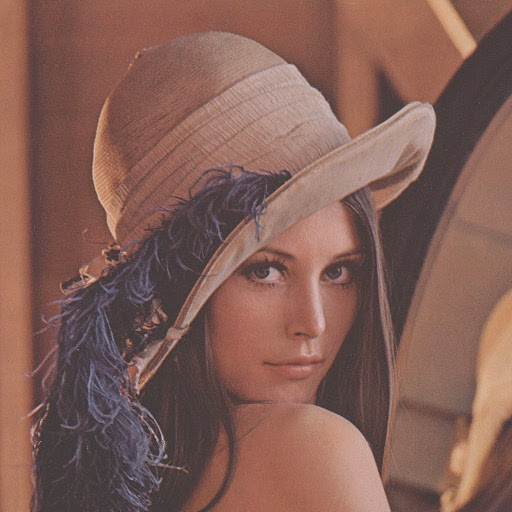
\includegraphics[width=3.5cm]{graphics/lenalc} \\
              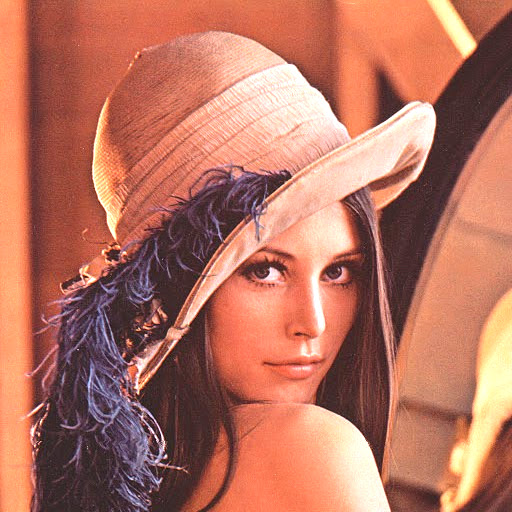
\includegraphics[width=3.5cm]{graphics/lenahc}
           \end{tabular}
           & \begin{tabular}{l}
             \parbox{0.6\linewidth}{%  change the parbox width as appropiate
             	
             		\begin{itemize}
             		\item La mejora del contraste es un proceso de transformación de la imagen, con el objetivo de obtener una nueva imagen con un contraste más definido.
					\item Se busca obtener imágenes más aptas para algún proceso posterior o toma de decisiones.
					\item La mejora del contraste es un área de investigación atractiva en el procesamiento de imágenes.
				    \end{itemize}

             }
         \end{tabular}  \\
\end{tabular}

\end{frame}

% \begin{frame}{Introducción}

% \begin{columns}[t]
% \begin{column}{.3\textwidth}
% \tcbox{\adjincludegraphics[width=0.85\linewidth,valign=t]{graphics/lena}}

% \end{column}
% \begin{column}{.7\textwidth}
% \begin{itemize}
% 	\item La mejora del contraste es un proceso de transformación de la imagen, con el objetivo de obtener una nueva imagen con un contraste más definido.
% 	\item Se busca obtener imágenes más aptas para algún proceso posterior.
% 	\item La mejora del contraste es un área de investigación atractiva en el procesamiento de imágenes.
% \end{itemize}
% % \hfill-- Carl Friedrich Gauss
% \end{column}
% \end{columns}
% \end{frame}
\begin{frame}{Introducción}
\begin{alertblock}{Problemática}
Mejora del Contraste automática de imágenes a color.
\end{alertblock}

\begin{columns}[t]
\begin{column}{.3\textwidth}
\tcbox{\adjincludegraphics[width=0.85\linewidth,valign=t]{graphics/lena}}

\end{column}
\begin{column}{.7\textwidth}
\begin{itemize}
	\item En las imágenes digitales en escala de gris solamente es necesario considerar la información representada por los niveles de intensidad de los pixeles.
	\item En las imágenes a color, es necesario además tener en cuenta la información de color representada, lo cual representa un problema adicional en el proceso.
\end{itemize}
% \hfill-- Carl Friedrich Gauss
\end{column}
\end{columns}
\end{frame}

\begin{frame}{Introducción}

\begin{columns}[t]
\begin{column}{.3\textwidth}
\tcbox{\adjincludegraphics[width=0.85\linewidth,valign=t]{graphics/lena}}

\end{column}
\begin{column}{.7\textwidth}
\begin{itemize}
	\item Una técnica importante para la Mejora del Contraste es la Ecualización del Histograma.
	\item Ésta técnica es directa y efectiva en el trabajo de Mejora del Contraste.
	\item Existen enfoques globales y locales de Ecualización del Histograma.
	\item Los enfoques locales son efectivos para el realce de detalles finos de la imagen digital.
\end{itemize}
% \hfill-- Carl Friedrich Gauss
\end{column}
\end{columns}


\end{frame}


\begin{frame}{Introducción}
\vspace{-0.5cm}
\begin{alertblock}{Objetivo}
Desarrollar un algoritmo para obtención de parámetros adecuados de Mejora del Contraste.
\end{alertblock}
\vspace{-0.2cm}
\begin{columns}[t]
\begin{column}{.3\textwidth}
\tcbox{\adjincludegraphics[width=0.85\linewidth,valign=t]{graphics/lena}}

\end{column}
\begin{column}{.7\textwidth}
\begin{itemize}
	\item En éste trabajo se busca atacar el problema de la Mejora del Contraste de imágenes digitales a color con un enfoque de Optimización Multi-Objetivo aplicado sobre un algoritmo de Ecualización del Histograma bien conocido.
	\item Se busca lograr un balance entre el realce de detalles de la imagen digital y el mantenimiento de la información de brillo y de color.
\end{itemize}
% \hfill-- Carl Friedrich Gauss
\end{column}
\end{columns}


\end{frame}


% \begin{frame}[fragile]
% \frametitle{Compiling}

% \begin{alertblock}{Warning}
% You can ignore this slide if you're working with Overleaf.
% \end{alertblock}

% To compile this deck you'll need the \texttt{biber} package. Probably your \TeX editor already supports it; if not, you will easily find online the instructions to install it.

% \vskip 0.5cm

% If you're not using an editor, you can compile this presentation using the command line by running:

% \begin{verbatim}
% $ pdflatex main.tex
% $ biber main.bcf
% $ pdflatex main.tex
% $ pdflatex main.tex
% \end{verbatim}


% \end{frame}

\section{Marco Teórico}

% \begin{frame}{Marco Teórico}

% \begin{columns}[t]
% \begin{column}{.3\textwidth}
% \tcbox{\adjincludegraphics[width=0.85\linewidth,valign=t]{graphics/lena}}

% \end{column}
% \begin{column}{.7\textwidth}
% \begin{itemize}
% 	\item Es necesario revisar dos partes:
% 	\begin{itemize}
% 		\item El proceso de Ecualización del Histograma,
% 		\item La Meta-Heurística Aplicada.
% 	\end{itemize}
% \end{itemize}
% % \hfill-- Carl Friedrich Gauss
% \end{column}
% \end{columns}


% \end{frame}

\begin{frame}{Marco Teórico}
\begin{alertblock}{Primeros pasos}
Separación de información de intensidad - Selección de espacios de color
\end{alertblock}
\vspace{-0.5cm}
\begin{columns}[t]
\begin{column}{.3\textwidth}
\tcbox{\adjincludegraphics[width=0.85\linewidth,valign=t]{graphics/lena}}
\end{column}
\begin{column}{.7\textwidth}
\begin{itemize}
	\item Se realiza una separación de la información de intensidad de la información de color para el proceso de ecualización del histograma.
	\item Se adoptaron representaciones de color bien conocidas para operar sobre la información de color de la imagen digital:
	\begin{itemize}
		\item $RGB$ (\textit{Red, Green, Blue})
		\item $YCbCr$
	\end{itemize}
\end{itemize}
% \hfill-- Carl Friedrich Gauss
\end{column}
\end{columns}
\end{frame}


% \begin{frame}{Colors}

% For this template we defined four colors, following the Style Manual of the University of Udine:
% \begin{itemize}
% \item \textcolor{white}{\marker{\texttt{UniOrange}}}
% \item \textcolor{white}{\marker[UniBlue]{\texttt{UniBlue}}}
% \item \textcolor{white}{\marker[UniBrown]{\texttt{UniBrown}}}
% \item \textcolor{white}{\marker[UniGold]{\texttt{UniGold}}}
% \end{itemize}

% \vskip 0.5cm

% You can use these colors as you want in your presentation. For example, you can \textbf{\textcolor{UniGold}{color the text in gold}} by writing \texttt{\textbackslash\{UniGold\}\{my gold text\}}.

% \vskip 0.5cm

% We also redefined many of the most common \LaTeX{} and Beamer commands, like \texttt{itemize}, \texttt{block}, etc. You will see samples of these commands in the following slides.

% \end{frame}

%\section{Blocks}

\begin{frame} 
\frametitle{Marco Teórico} 
% \framesubtitle{And also some blocks.} 
\begin{exampleblock}{\textit{Red, Green, Blue (RGB)}}
\end{exampleblock}

\begin{columns}[onlytextwidth]
\begin{column}{.45\textwidth}
\begin{figure}
  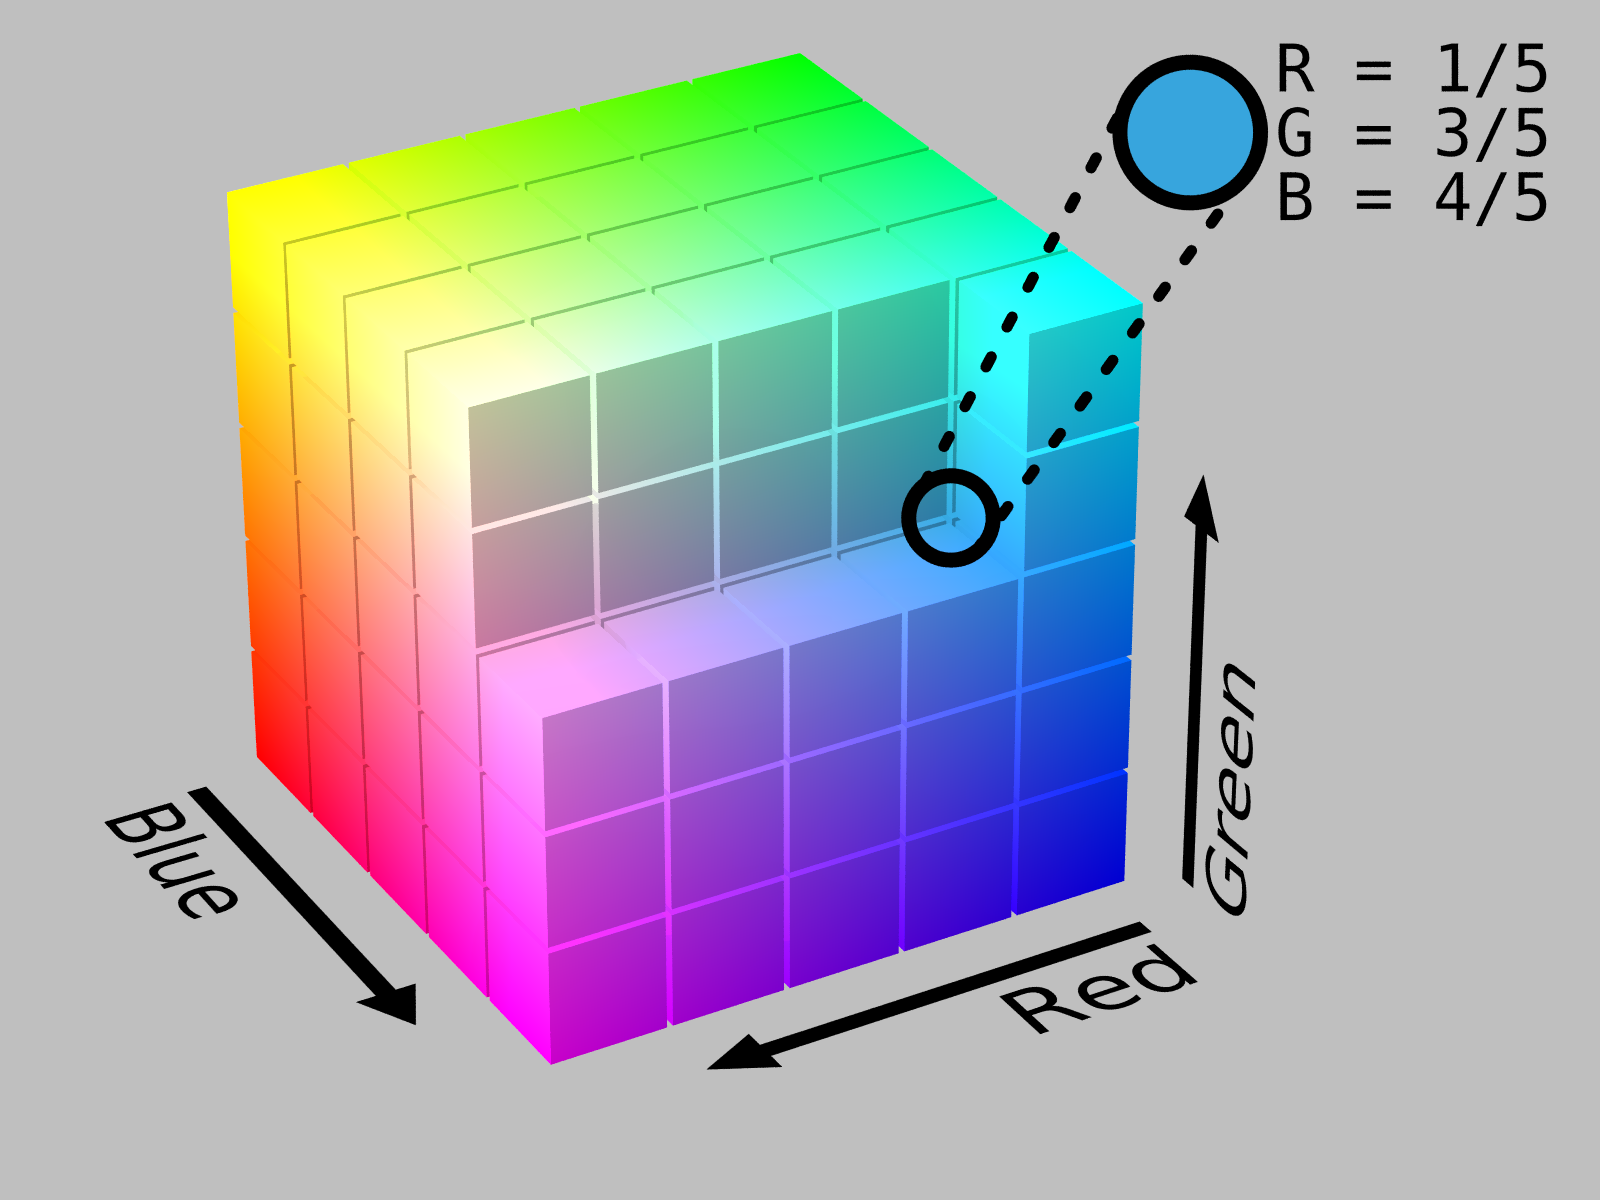
\includegraphics[width=4.5cm]{graphics/RGB_Cube_Show_lowgamma_cutout_b.png}
  \caption{$RGB$ es un espacio de representación de colores cartesiano}
\end{figure}
\end{column}
\hfill
\begin{column}{.45\textwidth}
    %             \begin{exampleblock}{\textit{Ventajas}}
				% \end{exampleblock}
             	
				Las imágenes digitales se representan inicialmente en $RGB$, por lo que se tiene un array de $N \times M \times 3$ pixeles de color.

				Cada pixel se representa como un elemento $[z_r \quad z_g \quad z_b]$ donde $z_r,z_g,z_b$ son los componentes de rojo, verde y azul del pixel a color en una ubicación específica.
\end{column}
\end{columns} 
%        \begin{tabular}{ll}  
%        	   \hspace{-1cm}
%            \begin{tabular}{l}
%               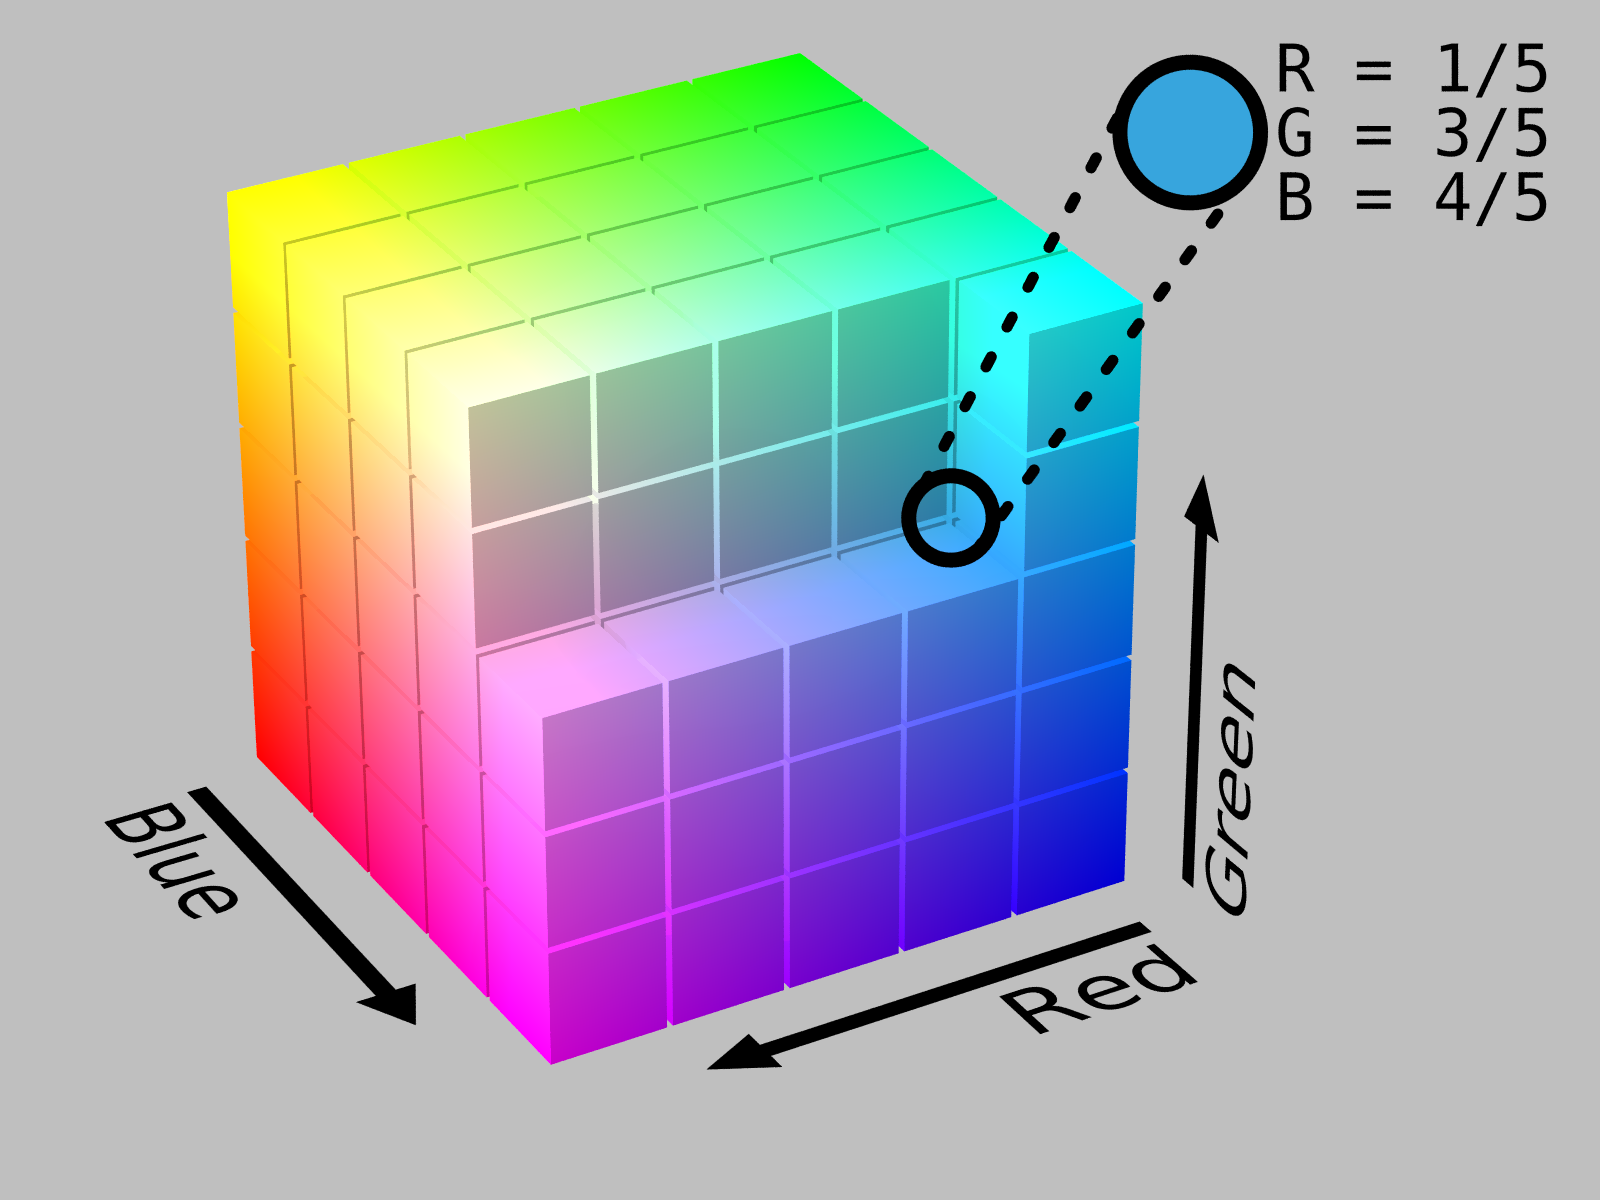
\includegraphics[width=4.5cm]{graphics/RGB_Cube_Show_lowgamma_cutout_b.png}
%            \end{tabular}
%            & \begin{tabular}{l}
%              \parbox{0.6\linewidth}{%  change the parbox width as appropiate
             	
% 				Las imágenes digitales se representan inicialmente en $RGB$, por lo que se tiene un array de $N \times M \times 3$ pixeles de color.

% 				Cada pixel se representa como un elemento $[z_r \quad z_g \quad z_b]$ donde $z_r,z_g,z_b$ son los componentes de rojo, verde y azul del pixel a color en una ubicación específica. Los componentes se mezclan para obtener el color representado por el pixel de la imagen.

%              }
%          \end{tabular}  \\
% \end{tabular}




% \centering
% \tcbox{\adjincludegraphics[width=0.25\linewidth,valign=t]{graphics/lena}}
% \adjincludegraphics[width=0.30\linewidth,valign=t]{graphics/RGB_Cube_Show_lowgamma_cutout_b}

\end{frame}

\begin{frame} 
\frametitle{Marco Teórico} 
% \framesubtitle{And also some blocks.} 
\begin{exampleblock}{\textit{Red, Green, Blue (RGB)}}
\end{exampleblock} 

\begin{columns}[onlytextwidth]
\begin{column}{.45\textwidth}
\begin{figure}
  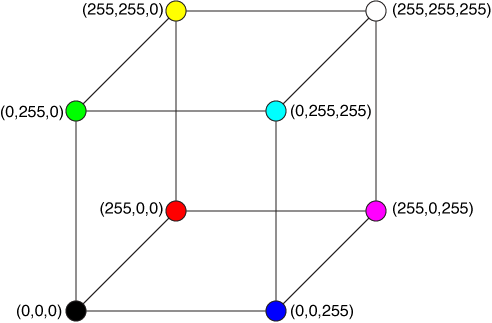
\includegraphics[width=\textwidth]{graphics/RGBCube.png}
  \caption{Representación de colores de ejemplo en el espacio $RGB$}
\end{figure}
\end{column}
\hfill
\begin{column}{.45\textwidth}
                \begin{exampleblock}{\textit{Ventajas}}
				\end{exampleblock}
             	
				\begin{itemize}
					\item Representación Sencilla
					\item Representación Bien conocida
					\item Implementación en varios lenguajes
				\end{itemize}
\end{column}
\end{columns}

% \centering
% \tcbox{\adjincludegraphics[width=0.25\linewidth,valign=t]{graphics/lena}}
% \adjincludegraphics[width=0.30\linewidth,valign=t]{graphics/RGB_Cube_Show_lowgamma_cutout_b}

\end{frame}


\begin{frame} 
\frametitle{Marco Teórico} 
% \framesubtitle{And also some blocks.} 
\begin{exampleblock}{\textit{YCbCr}}
\textit{YCbCr} es un espacio de color definido a través de una transformación matemática de coordenadas, a partir de un espacio de color $RGB$ asociado.

La ventaja de ésta representación es que separa la información de intensidades de la imagen digital de la información de color presente.
\end{exampleblock}

\centering
% \tcbox{\adjincludegraphics[width=0.25\linewidth,valign=t]{graphics/lena}}
% \adjincludegraphics[width=0.30\linewidth,valign=t]{graphics/RGB_Cube_Show_lowgamma_cutout_b}

\end{frame}

\begin{frame} 
\frametitle{Marco Teórico} 
% \framesubtitle{And also some blocks.} 
\vspace{-1cm}
\begin{figure}
  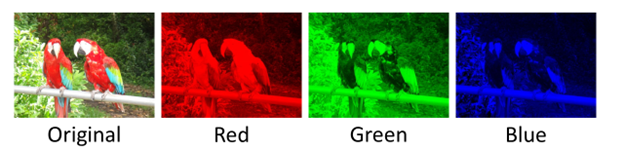
\includegraphics[width=11cm]{graphics/IC676790.png}
  \caption{Planos de componentes $rojo$, $verde$ y $azul$ en la representación $RGB$}
\end{figure}
\vspace{-1cm}
\begin{figure}
  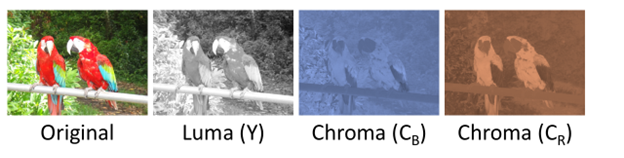
\includegraphics[width=11cm]{graphics/IC676791.png}
  \caption{Planos de componentes $Y$, $Cb$, $Cr$ en la representación $YCbCr$}
\end{figure}

% \tcbox{\adjincludegraphics[width=0.25\linewidth,valign=t]{graphics/lena}}
% \adjincludegraphics[width=0.30\linewidth,valign=t]{graphics/RGB_Cube_Show_lowgamma_cutout_b}

\end{frame}


\begin{frame} 
\frametitle{Marco Teórico} 
% \framesubtitle{And also some blocks.} 
\begin{exampleblock}{\textit{YCbCr}}
\textit{YCbCr} es un espacio de color definido a través de una transformación matemática de coordenadas, a partir de un espacio de color $RGB$ asociado.

Otra ventaja importante es que la conversión a partir de $RGB$, y luego de vuelta a $RGB$ es directa:
\end{exampleblock}
\vspace{-0.5cm}
\begin{equation}
\begin{bmatrix}
Y \\
C_b \\
C_r 
\end{bmatrix} =
\begin{bmatrix}
16  \\
128 \\
128
\end{bmatrix}
+
\begin{bmatrix}
65.481 & 128.553 & 24.966 \\
-37.797 & -74.203 & 112.000 \\
112.000 & -93.786 & -18.214 
\end{bmatrix}
\begin{bmatrix}
R \\
G \\
B 
\end{bmatrix}
\end{equation}
\begin{equation}
\begin{bmatrix}
R \\
G \\
B 
\end{bmatrix} =
\begin{bmatrix}
Y + 1.402 \cdot (C_r - 128) \\
Y -0.34414 \cdot (C_b - 128) - 0.71414 \cdot (C_r - 128) \\
Y + 1.772 \cdot  (C_b - 128) 
\end{bmatrix}
\end{equation}
\centering
% \tcbox{\adjincludegraphics[width=0.25\linewidth,valign=t]{graphics/lena}}
% \adjincludegraphics[width=0.30\linewidth,valign=t]{graphics/RGB_Cube_Show_lowgamma_cutout_b}

\end{frame}

\begin{frame} 
\frametitle{Marco Teórico} 
% \framesubtitle{And also some blocks.} 
\begin{exampleblock}{\textit{Contrast Limited Adaptive Histogram Equalization}}

Es un algoritmo de Mejora del Contraste de tipo local, diseñado para su aplicación en distintos tipos de imágenes. 

Sus parámetros de entrada principales consisten en:
\begin{equation}
\begin{split}
(\mathscr{R}_x, \mathscr{R}_y, \mathscr{C}) & \qquad (\mathscr{R}_x, \mathscr{R}_y) \in ([2,M/2],[2,N/2]) \\
											& \qquad \mathscr{C} \in [0,256]
\end{split}
\end{equation}


donde
\end{exampleblock}
\centering
% \tcbox{\adjincludegraphics[width=0.55\linewidth,valign=t]{graphics/Clahe-redist.jpg}}

\begin{itemize}
	\item $(\mathscr{R}_x, \mathscr{R}_y)$ son las dimensiones de la región de la imagen donde se realiza la Ecualización del Histograma.
	\item $\mathscr{C}$ es el coeficiente de recorte del histograma previo al proceso, \textit{Clip Limit}. 
\end{itemize}

% \tcbox{\adjincludegraphics[width=0.25\linewidth,valign=t]{graphics/lena}}
% \adjincludegraphics[width=0.30\linewidth,valign=t]{graphics/RGB_Cube_Show_lowgamma_cutout_b}

\end{frame}

\begin{frame} 
\frametitle{Marco Teórico} 
% \framesubtitle{And also some blocks.} 
\begin{exampleblock}{\textit{Entropía de la Imagen}}
\begin{itemize}

\item La Entropía de la imagen es una métrica que muestra la cantidad de información representada en la imagen digital.

\item La entropía de la imagen y su contraste están relacionados a la distribución de intensidad de las imágenes digitales, por lo que esta métrica es apta para medir variaciones del constraste como consecuencia de transformaciones aplicadas a la misma.

\end{itemize}

\end{exampleblock}
% \centering
% \tcbox{\adjincludegraphics[width=0.55\linewidth,valign=t]{graphics/Clahe-redist.jpg}}

\centering
% \tcbox{\adjincludegraphics[width=0.25\linewidth,valign=t]{graphics/lena}}
% \adjincludegraphics[width=0.30\linewidth,valign=t]{graphics/RGB_Cube_Show_lowgamma_cutout_b}

\end{frame}

% \begin{frame} 
% \frametitle{Marco Teórico} 
% % \framesubtitle{And also some blocks.} 
% \begin{exampleblock}{\textit{Efecto de la variación de Entropía de la Imagen}}

% \end{exampleblock}
% % \centering
% % \tcbox{\adjincludegraphics[width=0.55\linewidth,valign=t]{graphics/Clahe-redist.jpg}}

% \centering
% \begin{columns}[onlytextwidth]
% \begin{column}{.45\textwidth}
% \begin{figure}
%   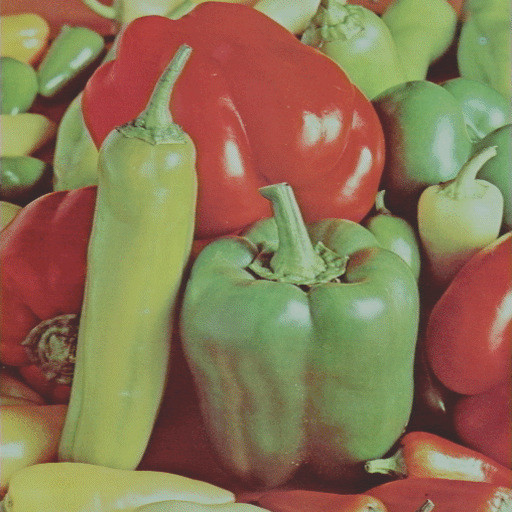
\includegraphics[width=\textwidth]{graphics/peppers_color_lc.jpg}
%   \caption{$\mathscr{H}=7,053228$}
% \end{figure}
% \end{column}
% \hfill
% \begin{column}{.45\textwidth}
% 		\begin{figure}
% 		  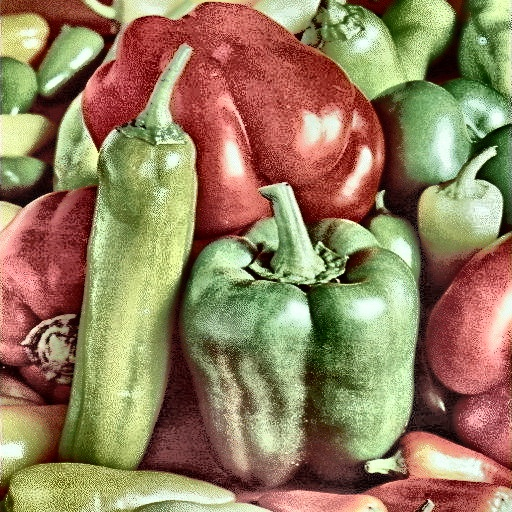
\includegraphics[width=\textwidth]{graphics/peppers_color_hc.jpg}
% 		  \caption{$\mathscr{H}=7,953866$}
% 		\end{figure}
% \end{column}
% \end{columns}

% \tcbox{\adjincludegraphics[width=0.25\linewidth,valign=t]{graphics/lena}}
% \adjincludegraphics[width=0.30\linewidth,valign=t]{graphics/RGB_Cube_Show_lowgamma_cutout_b}

% \end{frame}

\begin{frame} 
\frametitle{Marco Teórico} 
% \framesubtitle{And also some blocks.} 
\begin{exampleblock}{\textit{Efecto de la variación de Entropía de la Imagen}}

\end{exampleblock}
% \centering
% \tcbox{\adjincludegraphics[width=0.55\linewidth,valign=t]{graphics/Clahe-redist.jpg}}

\centering
\begin{columns}[onlytextwidth]
\begin{column}{.45\textwidth}
\begin{figure}
  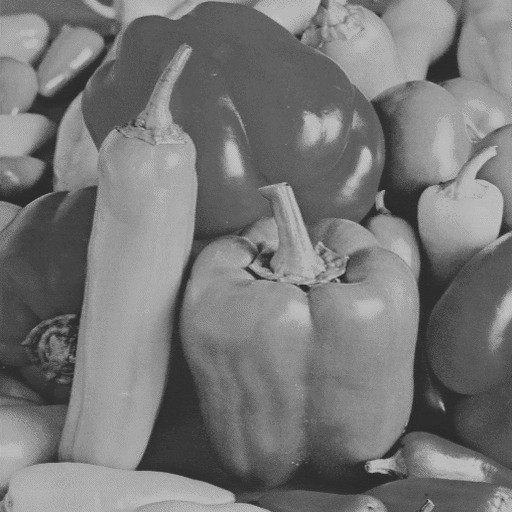
\includegraphics[width=\textwidth]{graphics/peppers_gray_lc.jpg}
  \caption{$\mathscr{H}=7,053228$}
\end{figure}
\end{column}
\hfill
\begin{column}{.45\textwidth}
		\begin{figure}
		  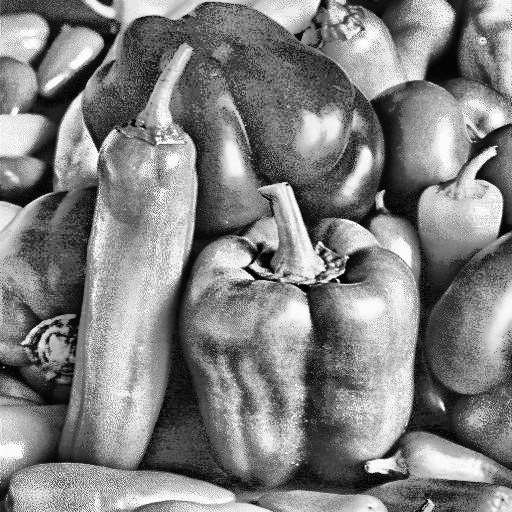
\includegraphics[width=\textwidth]{graphics/peppers_gray_hc.jpg}
		  \caption{$\mathscr{H}=7,953866$}
		\end{figure}
\end{column}
\end{columns}

% \tcbox{\adjincludegraphics[width=0.25\linewidth,valign=t]{graphics/lena}}
% \adjincludegraphics[width=0.30\linewidth,valign=t]{graphics/RGB_Cube_Show_lowgamma_cutout_b}
\end{frame}

\begin{frame} 
\frametitle{Marco Teórico} 
% \framesubtitle{And also some blocks.} 
\begin{exampleblock}{\textit{Efecto de la variación de Entropía de la Imagen}}

\end{exampleblock}
% \centering
% \tcbox{\adjincludegraphics[width=0.55\linewidth,valign=t]{graphics/Clahe-redist.jpg}}

\centering
\begin{columns}[onlytextwidth]
\begin{column}{.50\textwidth}
\begin{figure}
  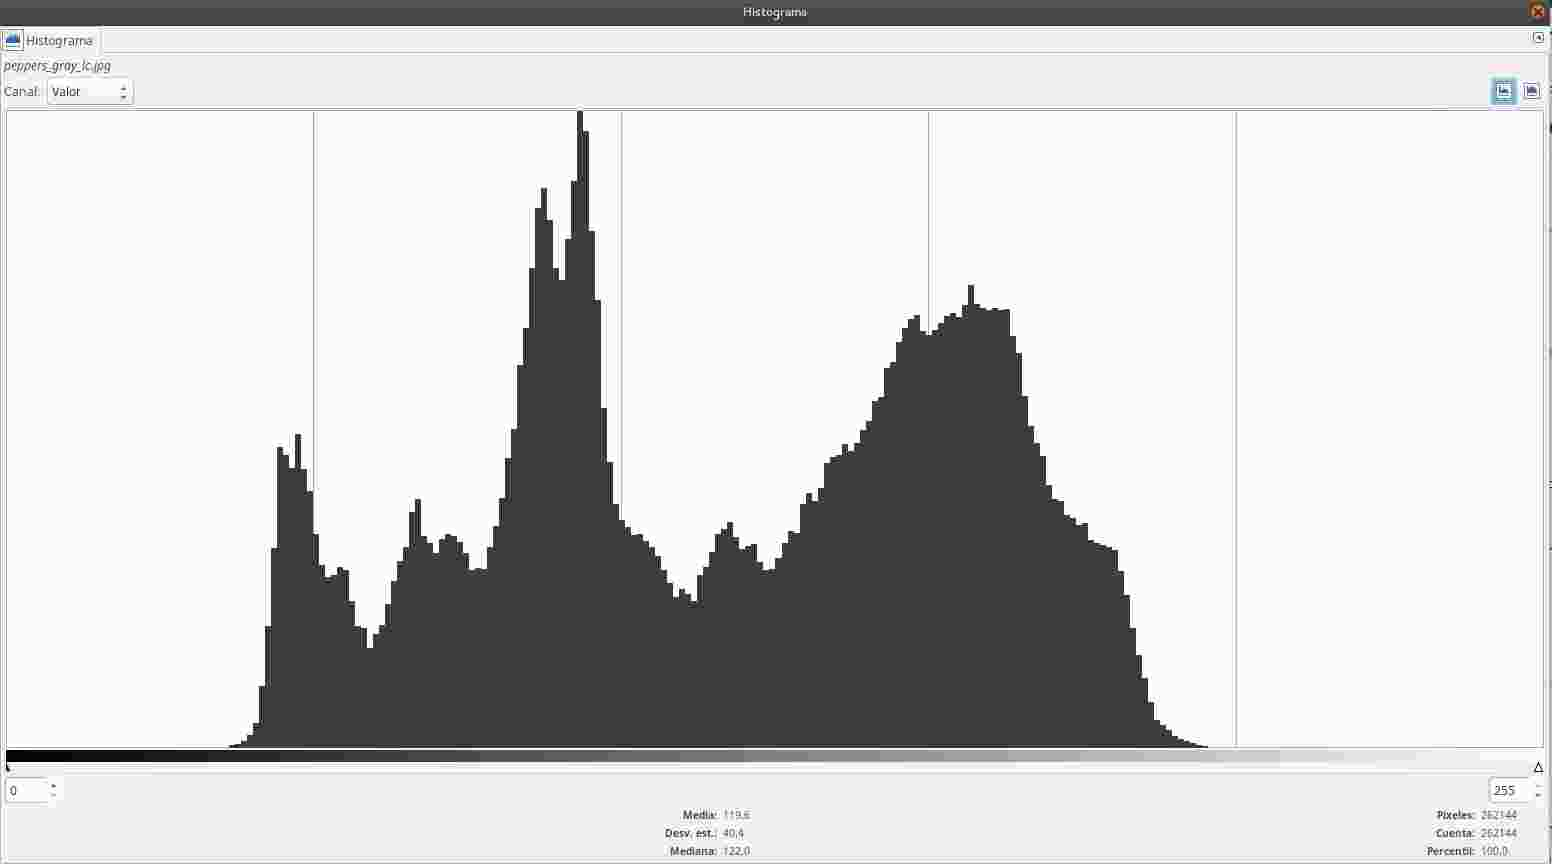
\includegraphics[width=\textwidth]{graphics/peppers_gray_lc_hist.jpg}
  \caption{$\mathscr{H}=7,053228$}
\end{figure}
\end{column}
\hfill
\begin{column}{.50\textwidth}
		\begin{figure}
		  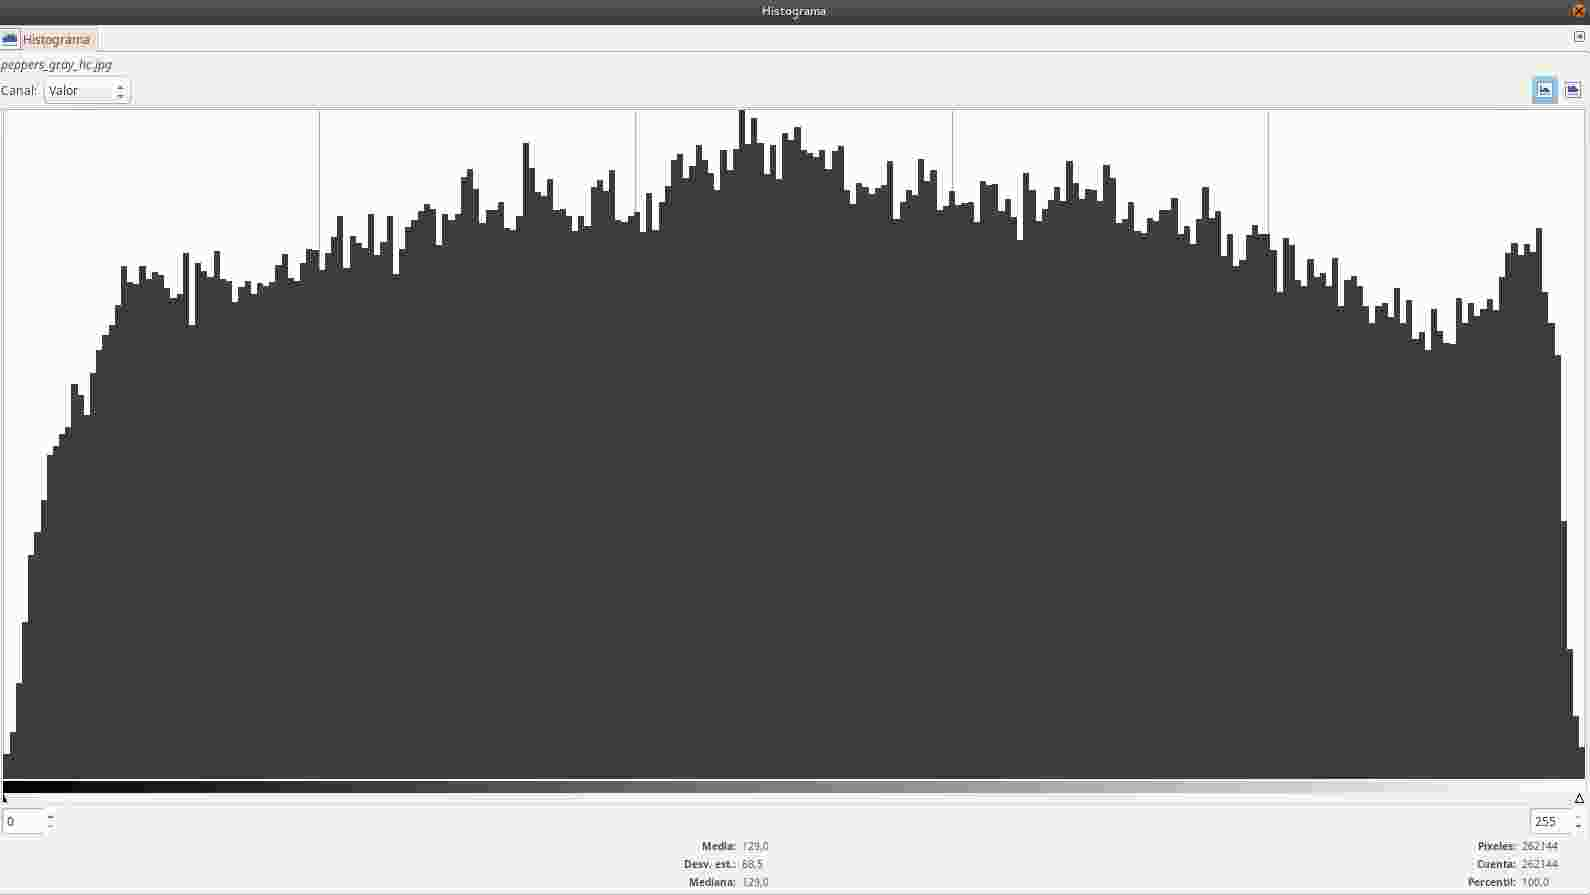
\includegraphics[width=\textwidth]{graphics/peppers_gray_hc_hist.jpg}
		  \caption{$\mathscr{H}=7,953866$}
		\end{figure}
\end{column}
\end{columns}

% \tcbox{\adjincludegraphics[width=0.25\linewidth,valign=t]{graphics/lena}}
% \adjincludegraphics[width=0.30\linewidth,valign=t]{graphics/RGB_Cube_Show_lowgamma_cutout_b}   
\end{frame}


\begin{frame} 
\frametitle{Marco Teórico} 
% \framesubtitle{And also some blocks.} 
\begin{exampleblock}{\textit{Entropía de la Imagen}}

La Entropía de la Imagen se define como se muestra abajo:

\end{exampleblock}

\begin{equation}
\mathscr{H}= -\sum_{i=0}^{L-1} p_i \text{log}_2(p_i) \qquad \mathscr{H} \in [0,\text{log}_2(L)]
\end{equation}

donde

\begin{equation}
p_i=\frac{c_i}{M \times N}, \qquad \sum_{i=1}^L c_i = M \times N, \qquad i= 1,2, ..., L
\end{equation}

$L$ es la cantidad de niveles de intensidad representables en la imagen, $M \times N$ es la cantidad de pixeles de la imagen.

\end{frame}    

\begin{frame} 

\frametitle{Marco Teórico} 
% \framesubtitle{And also some blocks.} 
\begin{exampleblock}{\textit{Structural Similarity Index}}
Es una métrica que mide atributos importantes de la imagen tales como la \textit{Luminancia, Contraste} y la \textit{Estructura}.

El objetivo de $SSIM$ es el de medir la distorsión de la imagen.

Dadas una imagen de entrada $I_x$ y una de salida $T_y$ $SSIM$ se define como se muestra abajo:

\end{exampleblock}
\vspace{-0.5cm}
\begin{equation}
SSIM(I,T) = \frac{(2\mu_{I_x} \mu_{T_y}+E_1)(2\sigma_{I_xT_y}+E_2)}{(\mu^2_{I_x}+\mu^2_{T_y}+E_1)(\sigma^2_{I_x} + \sigma^2_{T_y}+E_2)} \qquad SSIM \in [0,1]
\end{equation}

\begin{itemize}
	\item $\mu_{I_x}$ es el promedio de intensidades de los pixeles,
	\item $\sigma_{T_y}$ es la varianza intensidades de los pixeles,
	\item $\sigma_{I_xT_y}$ es el promedio de intensidades de los pixeles.
\end{itemize}

\end{frame}  

\begin{frame} 
\frametitle{Marco Teórico} 
% \framesubtitle{And also some blocks.} 
\begin{exampleblock}{\textit{Efecto de la variación de $SSIM$ de la Imagen}}

\end{exampleblock}
% \centering
% \tcbox{\adjincludegraphics[width=0.55\linewidth,valign=t]{graphics/Clahe-redist.jpg}}
\centering
\begin{columns}[onlytextwidth]
\begin{column}{.45\textwidth}
\begin{figure}
  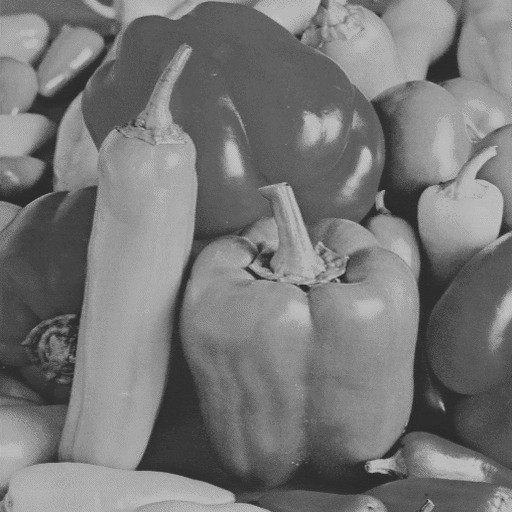
\includegraphics[width=\textwidth]{graphics/peppers_gray_lc.jpg}
  \caption{$SSIM_R=1 ; SSIM_G=1 ; SSIM_B=1$}
\end{figure}
\end{column}
\hfill
\begin{column}{.45\textwidth}
		\begin{figure}
		  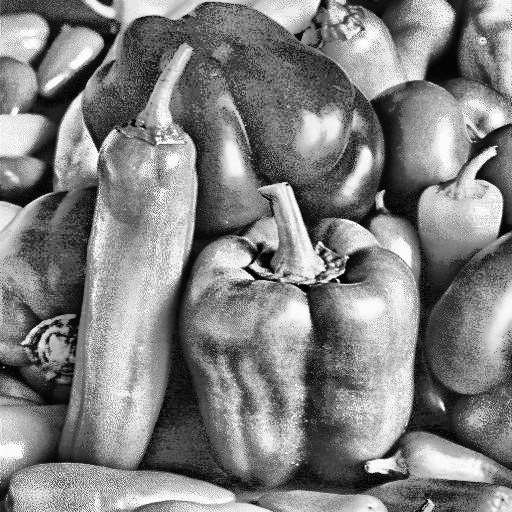
\includegraphics[width=\textwidth]{graphics/peppers_gray_hc.jpg}
		  \caption{$SSIM_R=0.484719; SSIM_G=0.525963; SSIM_B=0.533241$}
		\end{figure}
\end{column}
\end{columns}

% \tcbox{\adjincludegraphics[width=0.25\linewidth,valign=t]{graphics/lena}}
% \adjincludegraphics[width=0.30\linewidth,valign=t]{graphics/RGB_Cube_Show_lowgamma_cutout_b}
\end{frame}  

\begin{frame}
\frametitle{Marco Teórico} 
% \framesubtitle{And also some blocks.} 
\begin{exampleblock}{\textit{Multi-Objective Particle Swarm Optimization (MOPSO)}}

$MOPSO$ es una meta-heurística que emula el comportamiento social de las bandadas de pájaros.

Cada partícula $\vv{x}$ realiza una búsqueda dentro de un espacio $\Omega$, y para cada generación $t$, cada solución $\vv{x}$ se actualiza de acuerdo a:

\begin{equation}\label{eq:posicion1}
\vv{x}_i(t) = \vv{x}_i(t-1) + \vv{v}_i(t)
\end{equation}

Donde $\vv{v}$ se conoce como el factor de velocidad, y está dado por:

\begin{equation}\label{eq:velocidad1}
\vv{v}_i(t) = w \cdot (t-1) + C_1 \cdot r_1 \cdot (\vv{x}_{p_i} - \vv{x}_i) + C_2 \cdot r_2 \cdot (\vv{x}_{g_i} - \vv{x_i})
\end{equation}

\end{exampleblock}

% \begin{equation}
% SSIM(I,T) = \frac{(2\mu_{I_x} \mu_{T_y}+E_1)(2\sigma_{I_xT_y}+E_2)}{(\mu^2_{I_x}+\mu^2_{T_y}+E_1)(\sigma^2_{I_x} + \sigma^2_{T_y}+E_2)} \qquad SSIM \in [0,1]
% \end{equation}

\end{frame}

\begin{frame}
\frametitle{Marco Teórico} 
% \framesubtitle{And also some blocks.} 
\begin{exampleblock}{\textit{Multi-Objective Particle Swarm Optimization (MOPSO)}}

\begin{equation}\label{eq:velocidad1}
\vv{v}_i(t) = w \cdot (t-1) + C_1 \cdot r_1 \cdot (\vv{x}_{p_i} - \vv{x}_i) + C_2 \cdot r_2 \cdot (\vv{x}_{g_i} - \vv{x_i})
\end{equation}


Donde:

\begin{itemize}
\item $w$ es el peso de la inercia,
\item $C_1,C_2$ son parámetros específicos que controlan el efecto de las partículas locales y globales,
\item $r_1,r_2$ son variables aleatorias en el rango [0,1].
\end{itemize}


\end{exampleblock}
%         \label{fig:calhouse233orig}
%         \end{subfigure}
% \begin{subfigure}[]{
% 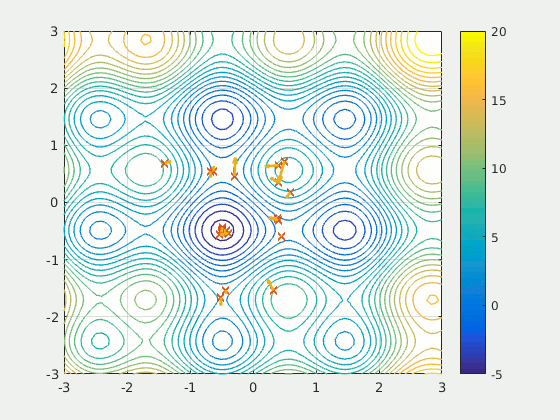
\includegraphics[width=0.45\textwidth]{./graphics/ejemplopso/capas-95.png}
% }
%     % \begin{subfigure}[t]{0.45\textwidth}
%         %\caption{Enhanced Image using \cite{morepso}. $\mathscr{H_Y}=0.788927$. $SSIM_R=0.000204143$. $SSIM_G=0.0000526475$. $SSIM_B=0.0000518143$}
%         \label{fig:calhouse23129}
%         \end{subfigure}
%     ~ %add desired spacing between images. e. g. ~. \quad. \qquad. \hfill etc. 
%     %(or a blank line to force the subfigure onto a new line)
%     \begin{subfigure}[]{
%     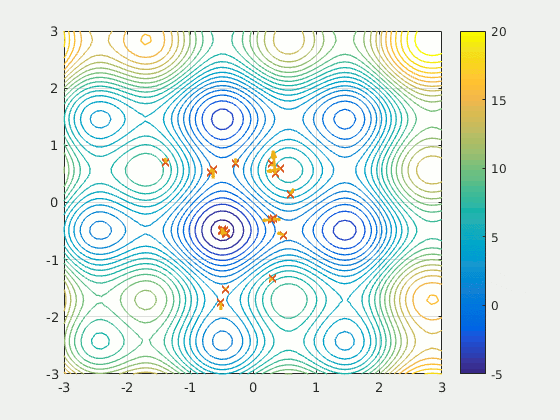
\includegraphics[width=0.45\textwidth]{./graphics/ejemplopso/capas-99.png}
%     }
%     % \begin{subfigure}[t]{0.45\textwidth}
% %        \caption{Enhanced Image.  $\mathscr{H_Y}=0.0350595$. $SSIM_R=0.416776$. $SSIM_G=0.403636$. $SSIM_B=0.417654$}
% \label{fig:calhouse231102}
% \end{subfigure}
%         \caption{Comportamiento de partículas en $PSO$ Monobjetivo a través de la serie de iteraciones. Nótese que las equis (x) indican un punto o solución potencial que se mueve sobre la superficie donde los colores más fríos son mejores soluciones.}
%         \label{fig:comportamientopso}
% \end{figure}

% \begin{equation}
% SSIM(I,T) = \frac{(2\mu_{I_x} \mu_{T_y}+E_1)(2\sigma_{I_xT_y}+E_2)}{(\mu^2_{I_x}+\mu^2_{T_y}+E_1)(\sigma^2_{I_x} + \sigma^2_{T_y}+E_2)} \qquad SSIM \in [0,1]
% \end{equation}

\end{frame}


\begin{frame}
\frametitle{Marco Teórico} 
% \framesubtitle{And also some blocks.} 
\begin{exampleblock}{\textit{Multi-Objective Particle Swarm Optimization (MOPSO)}}

\end{exampleblock}
\vspace{-0.5cm}
\begin{columns}[t]
\begin{column}{.45\textwidth}
\begin{figure}[H]
\centering
    %\begin{subfigure}[t]{0.45\textwidth}
    
    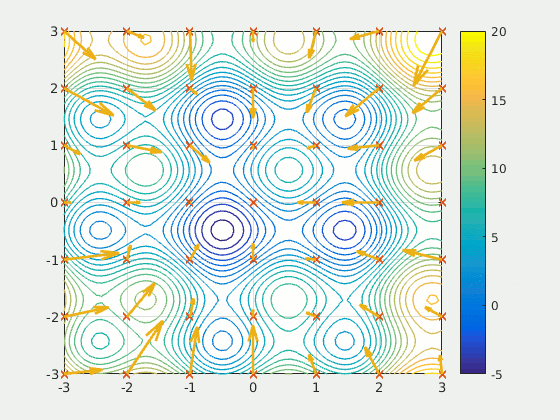
\includegraphics[width=\textwidth]{./graphics/ejemplopso/capas-0.png}
    
%        \caption{Imagen Original. $\mathscr{H_Y}=0.207231$. $SSIM_R=1$. $SSIM_G=1$. $SSIM_B=1$}
\end{figure}
\end{column}
\begin{column}{.45\textwidth}
    \begin{figure}[H]
        \centering
        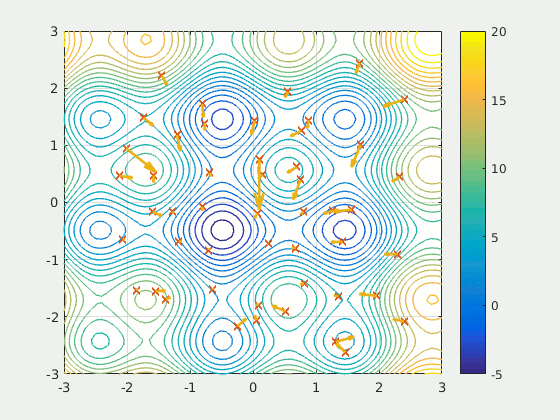
\includegraphics[width=\textwidth]{./graphics/ejemplopso/capas-8.png}   
    \end{figure}
\end{column}
\end{columns}
Comportamiento de partículas en $PSO$ Monobjetivo a través de la serie de iteraciones.
% \begin{figure}[H]
% \centering
%     %\begin{subfigure}[t]{0.45\textwidth}
% %     \begin{subfigure}[]{
% %     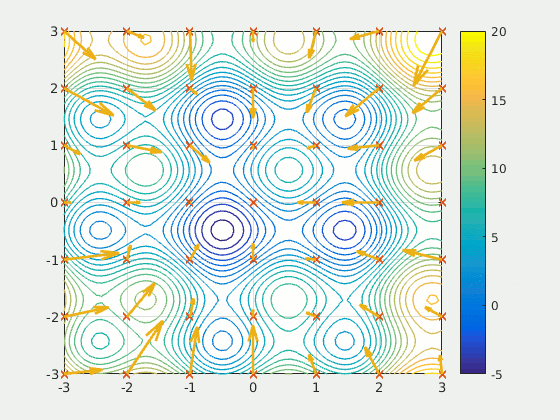
\includegraphics[width=0.45\textwidth]{./graphics/ejemplopso/capas-0.png}
% %     }
% % %        \caption{Imagen Original. $\mathscr{H_Y}=0.207231$. $SSIM_R=1$. $SSIM_G=1$. $SSIM_B=1$}
% % \end{subfigure}
%     % ~ %add desired spacing between images. e. g. ~. \quad. \qquad. \hfill etc. 
%       %(or a blank line to force the subfigure onto a new line)
% %       \begin{subfigure}[]{
% %       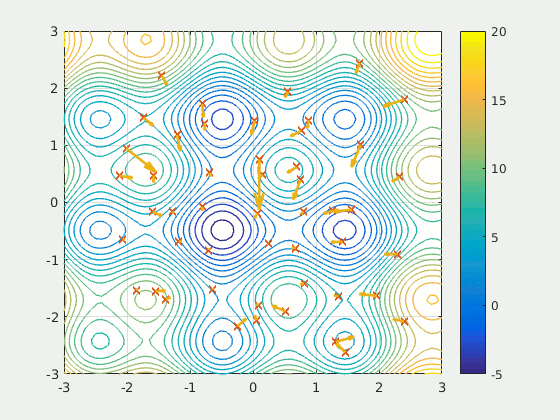
\includegraphics[width=0.45\textwidth]{./graphics/ejemplopso/capas-8.png}   
% %       }
% %     %\begin{subfigure}[t]{0.45\textwidth}
% % %        \caption{Enhanced Image. $\mathscr{H_Y}=0.611275$. $SSIM_R=0.00897331$. $SSIM_G=0.00823064$. $SSIM_B=0.00851013$}
% % \end{subfigure}
% %     ~ %add desired spacing between images. e. g. ~. \quad. \qquad. \hfill etc. 
%     %(or a blank line to force the subfigure onto a new line)
%     \begin{subfigure}[]{
%     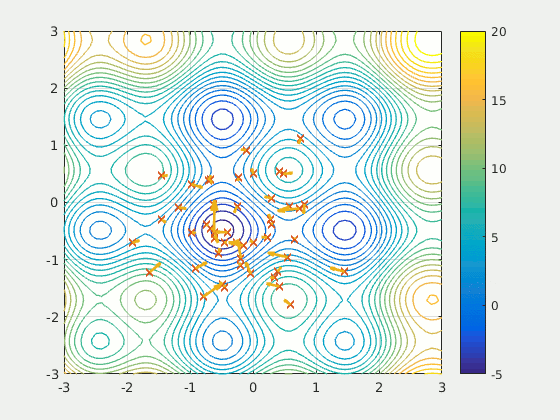
\includegraphics[width=0.45\textwidth]{./graphics/ejemplopso/capas-21.png}
%     }
%     % \begin{subfigure}[t]{0.45\textwidth}
% %        \caption{Enhanced Image.  $\mathscr{H_Y}=0.0350595$. $SSIM_R=0.416776$. $SSIM_G=0.403636$. $SSIM_B=0.417654$}
% \end{subfigure} 
% \begin{subfigure}[]{
% 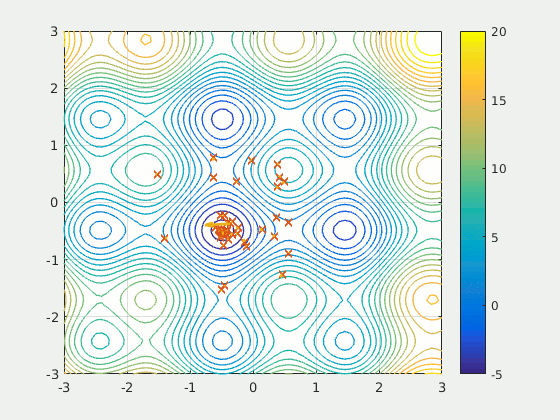
\includegraphics[width=0.45\textwidth]{./graphics/ejemplopso/capas-42.png}
% }
%     % \begin{subfigure}[t]{0.45\textwidth}
%         %\caption{Enhanced Image using \cite{morepso}. $\mathscr{H_Y}=0.788927$. $SSIM_R=0.000204143$. $SSIM_G=0.0000526475$. $SSIM_B=0.0000518143$}
%         \label{fig:calhouse23129}
%         \end{subfigure}
%     ~ %add desired spacing between images. e. g. ~. \quad. \qquad. \hfill etc. 
%     %(or a blank line to force the subfigure onto a new line)
%     \begin{subfigure}[]{
%     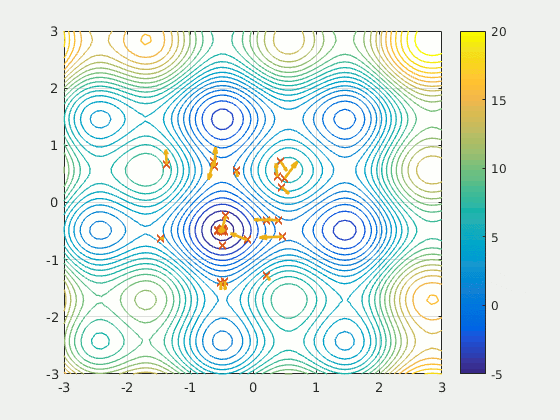
\includegraphics[width=0.45\textwidth]{./graphics/ejemplopso/capas-75.png}
%     }
%     % \begin{subfigure}[t]{0.45\textwidth}
% %        \caption{Enhanced Image.  $\mathscr{H_Y}=0.0350595$. $SSIM_R=0.416776$. $SSIM_G=0.403636$. $SSIM_B=0.417654$}
% \label{fig:calhouse231102}
% \end{subfigure} 
% \begin{subfigure}[]{
% 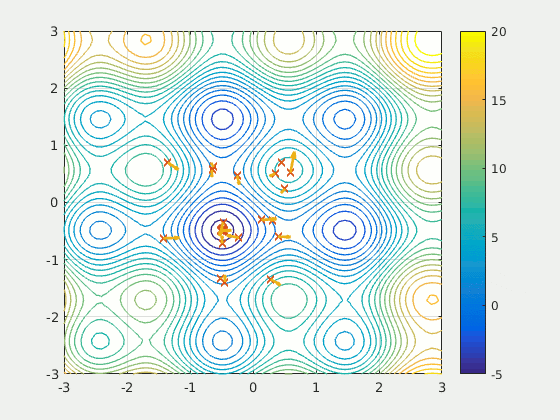
\includegraphics[width=0.45\textwidth]{./graphics/ejemplopso/capas-79.png}
% }
%     % \begin{subfigure}[t]{0.45\textwidth}
%         %\caption{Enhanced Image using \cite{morepso}. $\mathscr{H_Y}=0.788927$. $SSIM_R=0.000204143$. $SSIM_G=0.0000526475$. $SSIM_B=0.0000518143$}
%         \label{fig:calhouse233orig}
%         \end{subfigure}
% \begin{subfigure}[]{
% 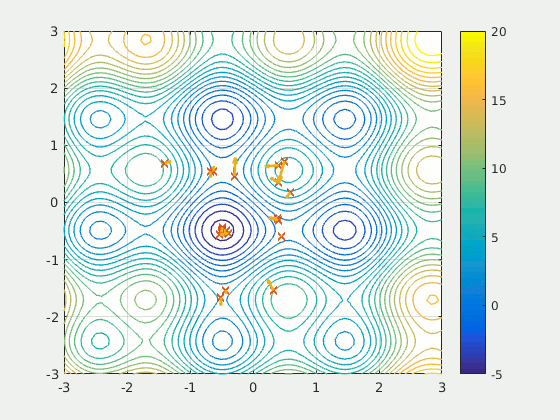
\includegraphics[width=0.45\textwidth]{./graphics/ejemplopso/capas-95.png}
% }
%     % \begin{subfigure}[t]{0.45\textwidth}
%         %\caption{Enhanced Image using \cite{morepso}. $\mathscr{H_Y}=0.788927$. $SSIM_R=0.000204143$. $SSIM_G=0.0000526475$. $SSIM_B=0.0000518143$}
%         \label{fig:calhouse23129}
%         \end{subfigure}
%     ~ %add desired spacing between images. e. g. ~. \quad. \qquad. \hfill etc. 
%     %(or a blank line to force the subfigure onto a new line)
%     \begin{subfigure}[]{
%     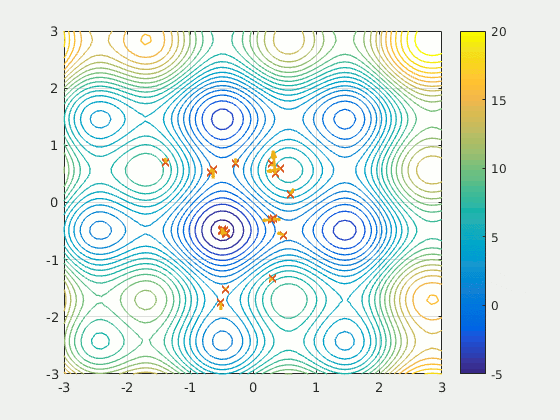
\includegraphics[width=0.45\textwidth]{./graphics/ejemplopso/capas-99.png}
%     }
%     % \begin{subfigure}[t]{0.45\textwidth}
% %        \caption{Enhanced Image.  $\mathscr{H_Y}=0.0350595$. $SSIM_R=0.416776$. $SSIM_G=0.403636$. $SSIM_B=0.417654$}
% \label{fig:calhouse231102}
% \end{subfigure}
%         \caption{Comportamiento de partículas en $PSO$ Monobjetivo a través de la serie de iteraciones. Nótese que las equis (x) indican un punto o solución potencial que se mueve sobre la superficie donde los colores más fríos son mejores soluciones.}
%         \label{fig:comportamientopso}
% \end{figure}

% \begin{equation}
% SSIM(I,T) = \frac{(2\mu_{I_x} \mu_{T_y}+E_1)(2\sigma_{I_xT_y}+E_2)}{(\mu^2_{I_x}+\mu^2_{T_y}+E_1)(\sigma^2_{I_x} + \sigma^2_{T_y}+E_2)} \qquad SSIM \in [0,1]
% \end{equation}

\end{frame}

\begin{frame}
\frametitle{Marco Teórico} 
% \framesubtitle{And also some blocks.} 
\begin{exampleblock}{\textit{Multi-Objective Particle Swarm Optimization (MOPSO)}}

\end{exampleblock}
\vspace{-0.5cm}
\begin{columns}[t]
\begin{column}{.45\textwidth}
\begin{figure}[H]
\centering
    %\begin{subfigure}[t]{0.45\textwidth}
    
    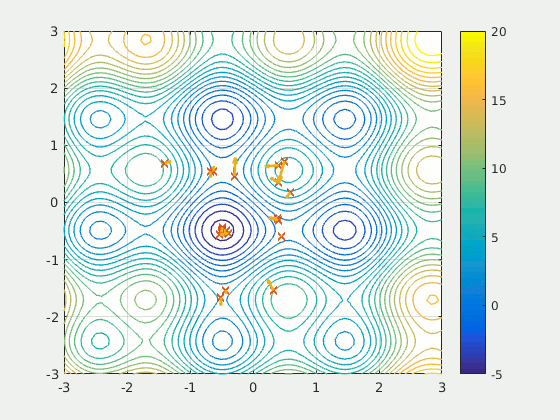
\includegraphics[width=\textwidth]{./graphics/ejemplopso/capas-95.png}
    
%        \caption{Imagen Original. $\mathscr{H_Y}=0.207231$. $SSIM_R=1$. $SSIM_G=1$. $SSIM_B=1$}
\end{figure}
\end{column}
\begin{column}{.45\textwidth}
    \begin{figure}[H]
        \centering
        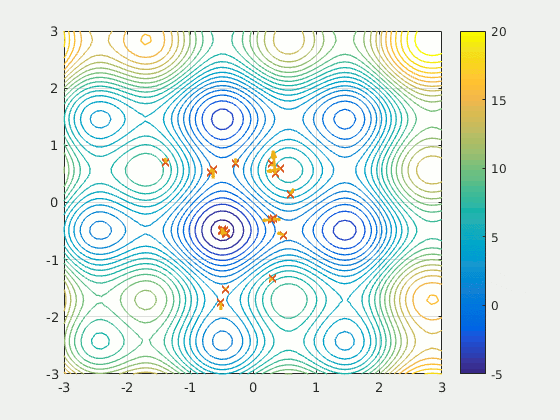
\includegraphics[width=\textwidth]{./graphics/ejemplopso/capas-99.png}   
    \end{figure}
\end{column}
\end{columns}
Comportamiento de partículas en $PSO$ Monobjetivo a través de la serie de iteraciones.
% \begin{figure}[H]
% \centering
%     %\begin{subfigure}[t]{0.45\textwidth}
% %     \begin{subfigure}[]{
% %     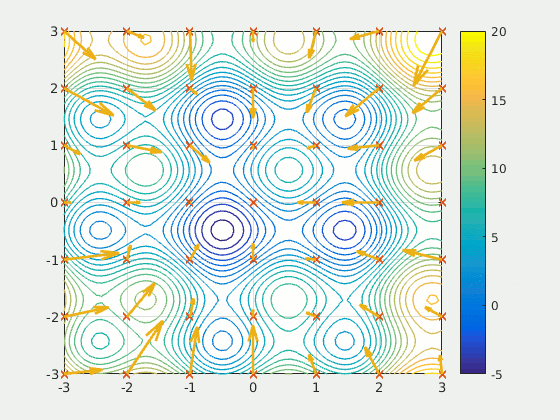
\includegraphics[width=0.45\textwidth]{./graphics/ejemplopso/capas-0.png}
% %     }
% % %        \caption{Imagen Original. $\mathscr{H_Y}=0.207231$. $SSIM_R=1$. $SSIM_G=1$. $SSIM_B=1$}
% % \end{subfigure}
%     % ~ %add desired spacing between images. e. g. ~. \quad. \qquad. \hfill etc. 
%       %(or a blank line to force the subfigure onto a new line)
% %       \begin{subfigure}[]{
% %       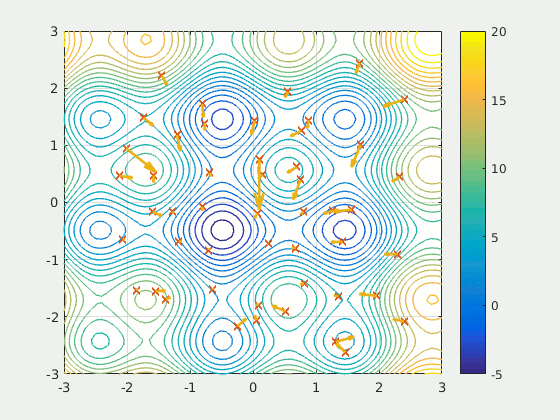
\includegraphics[width=0.45\textwidth]{./graphics/ejemplopso/capas-8.png}   
% %       }
% %     %\begin{subfigure}[t]{0.45\textwidth}
% % %        \caption{Enhanced Image. $\mathscr{H_Y}=0.611275$. $SSIM_R=0.00897331$. $SSIM_G=0.00823064$. $SSIM_B=0.00851013$}
% % \end{subfigure}
% %     ~ %add desired spacing between images. e. g. ~. \quad. \qquad. \hfill etc. 
%     %(or a blank line to force the subfigure onto a new line)
%     \begin{subfigure}[]{
%     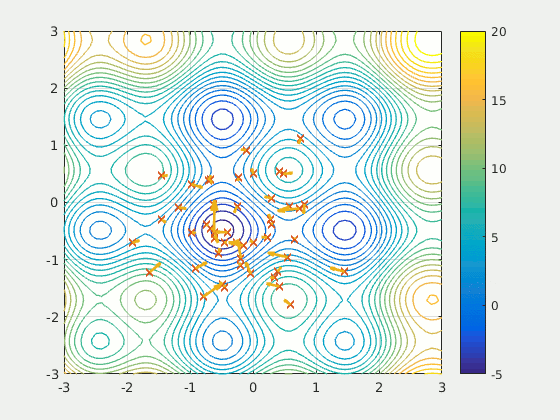
\includegraphics[width=0.45\textwidth]{./graphics/ejemplopso/capas-21.png}
%     }
%     % \begin{subfigure}[t]{0.45\textwidth}
% %        \caption{Enhanced Image.  $\mathscr{H_Y}=0.0350595$. $SSIM_R=0.416776$. $SSIM_G=0.403636$. $SSIM_B=0.417654$}
% \end{subfigure} 
% \begin{subfigure}[]{
% 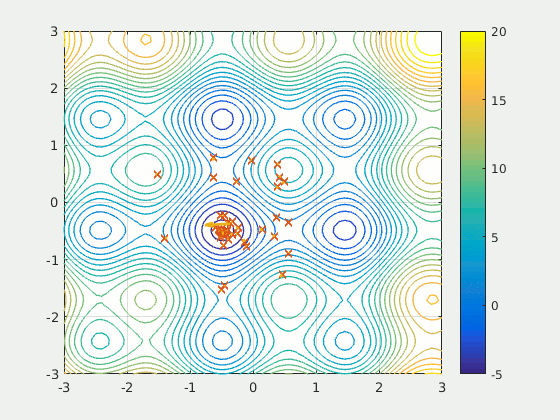
\includegraphics[width=0.45\textwidth]{./graphics/ejemplopso/capas-42.png}
% }
%     % \begin{subfigure}[t]{0.45\textwidth}
%         %\caption{Enhanced Image using \cite{morepso}. $\mathscr{H_Y}=0.788927$. $SSIM_R=0.000204143$. $SSIM_G=0.0000526475$. $SSIM_B=0.0000518143$}
%         \label{fig:calhouse23129}
%         \end{subfigure}
%     ~ %add desired spacing between images. e. g. ~. \quad. \qquad. \hfill etc. 
%     %(or a blank line to force the subfigure onto a new line)
%     \begin{subfigure}[]{
%     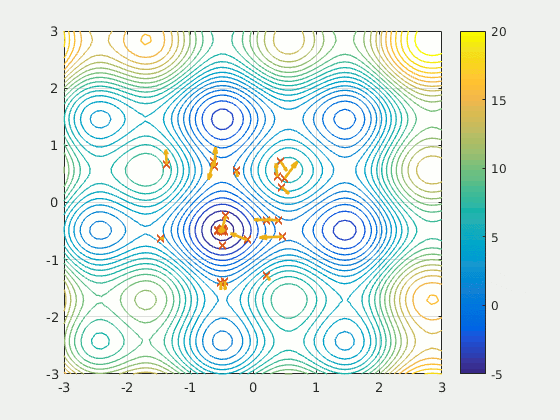
\includegraphics[width=0.45\textwidth]{./graphics/ejemplopso/capas-75.png}
%     }
%     % \begin{subfigure}[t]{0.45\textwidth}
% %        \caption{Enhanced Image.  $\mathscr{H_Y}=0.0350595$. $SSIM_R=0.416776$. $SSIM_G=0.403636$. $SSIM_B=0.417654$}
% \label{fig:calhouse231102}
% \end{subfigure} 
% \begin{subfigure}[]{
% 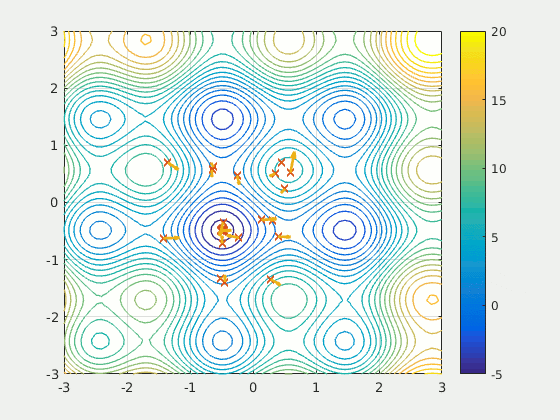
\includegraphics[width=0.45\textwidth]{./graphics/ejemplopso/capas-79.png}
% }
%     % \begin{subfigure}[t]{0.45\textwidth}
%         %\caption{Enhanced Image using \cite{morepso}. $\mathscr{H_Y}=0.788927$. $SSIM_R=0.000204143$. $SSIM_G=0.0000526475$. $SSIM_B=0.0000518143$}


% \begin{equation}
% SSIM(I,T) = \frac{(2\mu_{I_x} \mu_{T_y}+E_1)(2\sigma_{I_xT_y}+E_2)}{(\mu^2_{I_x}+\mu^2_{T_y}+E_1)(\sigma^2_{I_x} + \sigma^2_{T_y}+E_2)} \qquad SSIM \in [0,1]
% \end{equation}

\end{frame}


\section{Formulación del Problema Planteado}

\begin{frame}
\frametitle{Formulación del Problema Planteado} 
% \framesubtitle{And also some blocks.} 
\begin{exampleblock}{\textit{Formulación del Problema Planteado}}

Dada una imagen a color $I$, con $M \times N$ pixeles, se busca un conjunto de soluciones no dominadas $\mathscr{X}$, que maximiza simultáneamente las funciones objetivo $f_1,f_2,f_3,f_4$:

\begin{equation}
\begin{split}
\mathscr{P} &= (\mathscr{X}) \longrightarrow \text{max}[f_1(T_y),f_2(I_R,T_R),f_3(I_G,T_G),f_4(I_B,T_B)]; \\
            & \qquad f_1,f_2,f_3,f_4 \in [0,1]
\end{split}
\end{equation}

\end{exampleblock}

donde

\begin{itemize}
        \item $I$ es la imagen a la que se aplica el proceso de Mejora del Contraste, y $T$\label{symbol:imejorada} es una de las imágenes resultantes del proceso,
\end{itemize}

% \begin{equation}
% SSIM(I,T) = \frac{(2\mu_{I_x} \mu_{T_y}+E_1)(2\sigma_{I_xT_y}+E_2)}{(\mu^2_{I_x}+\mu^2_{T_y}+E_1)(\sigma^2_{I_x} + \sigma^2_{T_y}+E_2)} \qquad SSIM \in [0,1]
% \end{equation}

\end{frame}

\begin{frame}
\frametitle{Formulación del Problema Planteado} 
% \framesubtitle{And also some blocks.} 
% \begin{exampleblock}{\textit{Formulación del Problema Planteado}}

\begin{equation}
\begin{split}
\mathscr{P} &= (\mathscr{X}) \longrightarrow \text{max}[f_1(T_y),f_2(I_R,T_R),f_3(I_G,T_G),f_4(I_B,T_B)]; \\
            & \qquad f_1,f_2,f_3,f_4 \in [0,1]
\end{split}
\end{equation}

% \end{exampleblock}

donde

\begin{itemize}
	\item $T_y$ es el mapa de intensidades mejoradas, al aplicar $\vv{x}$ a $I_y$; ésto es: $T_y=CLAHE(\vv{x},I_y\label{symbol:ioriginaly})$. $T_y$ e $I_y$ son los canales $Y$ de la representación $YCbCr$  de las imágenes $I$ y $T$, respectivamente,
	\item $f_1(T_y)\label{symbol:imejoraday}=\frac{\mathscr{H}(T_y)}{\text{log}_2L}$ es la Entropía Normalizada del mapa de intensidades mejoradas $T_y$
	\item $f_2(I_R\label{symbol:ioriginalr},T_R\label{symbol:imejoradar})=SSIM(I_R,T_R)$ es la medición del $SSIM$ entre $I_R$ y $T_R$. $I_R$ y $T_R$ son los canales $R$ de las representaciones $RGB$ de $I$ y $T$, respectivamente,
	% \item $f_2(I_G\label{symbol:ioriginalg},T_G\label{symbol:imejoradag})=SSIM(I_G,T_G)$ es la medición del $SSIM$ entre $I_G$ y $T_G$. $I_G$ y $T_G$ son los canales $G$ de las representaciones $RGB$ de $I$ y $T$, respectivamente,
	% \item $f_2(I_B\label{symbol:ioriginalb},T_B\label{symbol:imejoradab})=SSIM(I_B,T_B)$ es la medición del $SSIM$ entre $I_B$ y $T_B$. $I_B$ y $T_B$ son los canales $G$ de las representaciones $RGB$ de $I$ y $T$, respectivamente,
\end{itemize}

% Acotados por:

% %Bounded to:

% \begin{itemize}
% 	\item $\mathscr{R}_x \in [2,...,M]$ dentro de $\mathbb{N}$,
% 	\item $\mathscr{R}_y \in [2,...,N]$ dentro de $\mathbb{N}$,
% 	\item $\mathscr{C} \in (0,...,1]$ dentro $\mathbb{R}$.
% \end{itemize}

% \begin{equation}
% SSIM(I,T) = \frac{(2\mu_{I_x} \mu_{T_y}+E_1)(2\sigma_{I_xT_y}+E_2)}{(\mu^2_{I_x}+\mu^2_{T_y}+E_1)(\sigma^2_{I_x} + \sigma^2_{T_y}+E_2)} \qquad SSIM \in [0,1]
% \end{equation}

\end{frame}

\begin{frame}
\frametitle{Formulación del Problema Planteado} 
% \framesubtitle{And also some blocks.} 
% \begin{exampleblock}{\textit{Formulación del Problema Planteado}}

\begin{equation}
\begin{split}
\mathscr{P} &= (\mathscr{X}) \longrightarrow \text{max}[f_1(T_y),f_2(I_R,T_R),f_3(I_G,T_G),f_4(I_B,T_B)]; \\
            & \qquad f_1,f_2,f_3,f_4 \in [0,1]
\end{split}
\end{equation}

% \end{exampleblock}

donde

\begin{itemize}
	\item $f_2(I_G\label{symbol:ioriginalg},T_G\label{symbol:imejoradag})=SSIM(I_G,T_G)$ es la medición del $SSIM$ entre $I_G$ y $T_G$. $I_G$ y $T_G$ son los canales $G$ de las representaciones $RGB$ de $I$ y $T$, respectivamente,
	\item $f_2(I_B\label{symbol:ioriginalb},T_B\label{symbol:imejoradab})=SSIM(I_B,T_B)$ es la medición del $SSIM$ entre $I_B$ y $T_B$. $I_B$ y $T_B$ son los canales $G$ de las representaciones $RGB$ de $I$ y $T$, respectivamente,
\end{itemize}

%Bounded to:

\begin{itemize}
	\item $\mathscr{R}_x \in [2,...,M]$ dentro de $\mathbb{N}$,
	\item $\mathscr{R}_y \in [2,...,N]$ dentro de $\mathbb{N}$,
	\item $\mathscr{C} \in (0,...,1]$ dentro $\mathbb{R}$.
\end{itemize}

% \begin{equation}
% SSIM(I,T) = \frac{(2\mu_{I_x} \mu_{T_y}+E_1)(2\sigma_{I_xT_y}+E_2)}{(\mu^2_{I_x}+\mu^2_{T_y}+E_1)(\sigma^2_{I_x} + \sigma^2_{T_y}+E_2)} \qquad SSIM \in [0,1]
% \end{equation}

\end{frame}

% \subsection{Enumerates and itemizes}

% \begin{frame}{Enumerates and itemizes}

% This is an example of \texttt{itemize}.
% \begin{itemize}
% 	\item A long time ago in a galaxy far, far away...
% \end{itemize}
% And this is an example of \texttt{enumerate}.

% \begin{enumerate} 
%   \item Go to the Death Star.
%   \item Find the exhaust port.
%   \item Make the perfect shot.
%   \item Become an hero.
% \end{enumerate}
% \end{frame}

% \subsection{Description}

% \begin{frame}[fragile]
% \frametitle{Description}
% This is an example of \texttt{description}.

% \begin{description}
% \item<2->[Vader] \emph{I am} your father.
% \item<1->[Luke] No. No! That's not true! \textbf{That's impossible!}
% \end{description}

% \begin{uncoverenv}<3>
%   \vskip 0.5cm
%   And while we're here, let's have a look to \texttt{verbatim} as well, to see how we made items appear in arbitrary order:
%   \vskip 0.5cm
%   \begin{verbatim}
% \begin{description}
%   \item<2->[This is the first item] one
%   \item<1->[This is the second item] two
% \end{description}
%   \end{verbatim}
% \end{uncoverenv}

% \end{frame}

\section{Propuesta}

\begin{frame}
\frametitle{Propuesta - CMOPSO-CLAHE} 
% \framesubtitle{And also some blocks.} 
\begin{exampleblock}{\textit{Diagrama esquemático de CMOPSO - CLAHE}}

\end{exampleblock}

\begin{figure}[H]
\centering
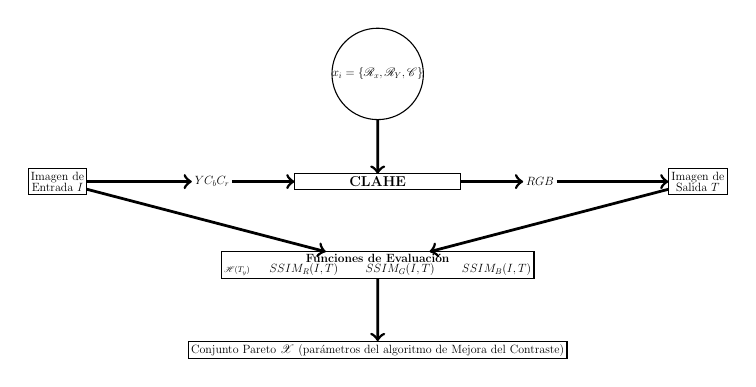
\begin{tikzpicture}[scale=0.3, transform shape]

%textos

%\node[draw,align=center] at (3,4) {\textbf{MANY-PSO-CLAHE}};
                                   
\node[draw,align=center,minimum width=200pt] (manypsoclahe) {\LARGE \textbf{CLAHE}};

\node[draw,align=center,below= 75pt of manypsoclahe] (evaluationfunctions) {\Large \textbf{Funciones de Evaluación}\\ $\mathscr{H}(T_y)$ \qquad \Large $SSIM_R(I,T)$ \qquad $SSIM_G(I,T)$ \qquad $SSIM_B(I,T)$};
                                   
\node[draw,align=center,below= 75pt of evaluationfunctions] (paretoset) {\Large Conjunto Pareto $\mathscr{X}$ (parámetros del algoritmo de Mejora del Contraste)};

\node[draw,align=center,left= 250pt of manypsoclahe] (inputimage) {\Large Imagen de \\ \Large Entrada $I$};

\node[draw,align=center,right= 250pt of manypsoclahe] (outputimage) {\Large Imagen de \\ \Large Salida $T$};

% \node[draw,circle,minimum size=1cm,inner sep=0pt,above left= 65pt and -40pt of manypsoclahe] (partic1) {\small $\mathscr{R}_x,\mathscr{R}_Y,\mathscr{C}$};

\node[draw,circle,minimum size=1cm,inner sep=0pt,above = 65pt of manypsoclahe] (partic2) {\Large $\vv{x_i}=\{\mathscr{R}_x,\mathscr{R}_Y,\mathscr{C}\}$};

% \node[draw,circle,minimum size=1cm,inner sep=0pt,above right= 65pt and -40pt of manypsoclahe] (partic3) {\small $\mathscr{R}_x,\mathscr{R}_Y,\mathscr{C}$};

\node[align=center,left= 75pt of manypsoclahe] (ycrcb) {\Large $YC_bC_r$};

\node[align=center,right= 75pt of manypsoclahe] (rgb) {\Large $RGB$};

\draw[->,draw=black,line width=1pt]
  % (partic1) edge (manypsoclahe) 
  (partic2) edge (manypsoclahe)
  % (partic3) edge (manypsoclahe)
  (inputimage) edge (ycrcb)
  (ycrcb) edge (manypsoclahe)
  (manypsoclahe) edge (rgb)
  (rgb) edge (outputimage)
  (outputimage) edge (evaluationfunctions)
  (inputimage) edge (evaluationfunctions)
  (evaluationfunctions) edge (paretoset);

\end{tikzpicture}
\caption{Proceso de evaluación de una solución potencial, para una iteración $t$ de la implementación.}
\label{fig:interaccioncmopsoclahe}
\end{figure}

\end{frame}

% \begin{frame}{Maths}
% A formula will look like this: 
% \begin{center}
%  $x^2 + y^2 = z^2$
% \end{center}

% You can number equations as well:
% \begin{equation}
% 1+1=2
% \end{equation}

% \begin{equation}
% 1+1=2 \tag{custom label!}
% \end{equation}

% \vskip 0.5cm

% If you want to use the default \LaTeX{} math fonts, just go to \texttt{beamerfontthemeuniud.sty} and uncomment the line containing `\texttt{\textbackslash usefonttheme[onlymath]\{serif\}}'.

% \end{frame}

% \begin{frame}{Theorems}

% The usual \texttt{theorem}, \texttt{corollary}, \texttt{definition}, \texttt{definitions}, \texttt{fact}, \texttt{example} and \texttt{examples} blocks are available as well.

% \begin{theorem}
% There exists an infinite set.
% \end{theorem}
% \begin{proof}
% This follows from the axiom of infinity.
% \end{proof}
% \begin{example}[Natural Numbers]
% The set of natural numbers is infinite.
% \end{example}

% \end{frame}

\section{Resultados y discusión}

\begin{frame}
\frametitle{Resultados y discusión} 
% \framesubtitle{And also some blocks.} 
\begin{exampleblock}{\textit{Parámetros Iniciales }}

\end{exampleblock}

\begin{table}[H]
\setlength{\abovecaptionskip}{2pt plus 3pt minus 2pt} % Chosen fairly arbitrarily
\caption[Parámetros de entrada para $MOPSO$]{Parámetros iniciales para $CMOPSO-CLAHE$}
\begin{center}
\begin{tabular}{||c c | c c||} 
\hline
Parámetro & Valor & Parámetro & Valor \\ [0.5ex] 
\hline\hline
$M$ & $256$ & $N$ & $256$ \\ 
\hline
$lower\_limit_{\mathscr{R}_x}$ & $2$ & $upper\_limit_{\mathscr{R}_x}$ & $M/2$ \\ 
\hline
$lower\_limit_{\mathscr{R}_y}$ & $2$ & $upper\_limit_{\mathscr{R}_y}$ & $N/2$ \\  
\hline
$lower\_limit_{{\mathscr{C}}}$ & $0$ & $upper\_limit_{{\mathscr{C}}}$ & 0.5 \\
\hline
$\Omega$ & $100$ & $t_{max}$ & $100$ \\ 
\hline
$c_1$ $min$ & 1.5 & $c_1$ $max$ & 2.5 \\ 
\hline
$c_2$ $min$ & 1.5 & $c_2$ $max$ & 2.5 \\ 
\hline
$r_1$ $min$ & 0.0 & $r_1$ $max$ & 1.0 \\ 
\hline
$r_2$ $min$ & 0.0 & $r_2$ $max$ & 1.0 \\
\hline
\end{tabular}
\end{center}
\label{table:parametrospso}
\end{table}

\end{frame}

\begin{frame}
\frametitle{Resultados y discusión} 
% \framesubtitle{And also some blocks.} 

\begin{figure}[H]
\centering
\begin{subfigure}[t]{0.45\textwidth}
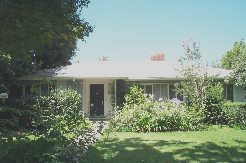
\includegraphics[width=\textwidth]{graphics/calhouse_0230.jpg}
\caption{Imagen Original. $\mathscr{H_Y}=7,792769$, $SSIM_R=1$, $SSIM_G=1$, $SSIM_B=1$}
\label{fig:casa1original}
\end{subfigure}
    ~ %add desired spacing between images, e. g. ~, \quad, \qquad, \hfill etc. 
      %(or a blank line to force the subfigure onto a new line)
      \begin{subfigure}[t]{0.45\textwidth}
      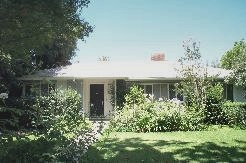
\includegraphics[width=\textwidth]{graphics/calhouse_0230_20-25165283474-10.jpg}
      \caption{Imagen Contrastada utilizando $CMOPSO-CLAHE$. $\mathscr{H_Y}=7,388725$, $SSIM_R=0,99102669$, $SSIM_G=0,99176936$, $SSIM_B=0,99148987$}
      \label{fig:casa1enhanced1}
      \end{subfigure} \\
    % ~ %add desired spacing between images, e. g. ~, \quad, \qquad, \hfill etc. 
    % %(or a blank line to force the subfigure onto a new line)
    % \begin{subfigure}[t]{0.45\textwidth}
    %     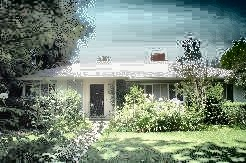
\includegraphics[width=\textwidth]{graphics/calhouse_0230_20-62968204656-00.jpg}
    %     \caption{Enhanced Image.  $\mathscr{H_Y}=0.0350595$, $SSIM_R=0.416776$, $SSIM_G=0.403636$, $SSIM_B=0.417654$}
    %     \label{fig:casa1enhanced2}
    % \end{subfigure} 
    % \begin{subfigure}[t]{0.45\textwidth}
    %     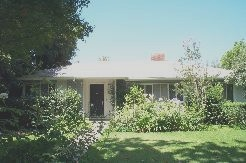
\includegraphics[width=\textwidth]{graphics/calhouse_0230_20-20-0020072469292179818.jpg}
    %     \caption{Enhanced Image using \cite{morepso}. $\mathscr{H_Y}=0.788927$, $SSIM_R=0.000204143$, $SSIM_G=0.0000526475$, $SSIM_B=0.0000518143$}
    %     \label{fig:casa1enhanced3}
    % \end{subfigure}

    \caption{Imágenes original y contrastadas para \texttt{calhouse\_230.jpg}}\label{fig:casa1}
    \end{figure}

    \end{frame}


    \begin{frame}
    \frametitle{Resultados y discusión} 
% \framesubtitle{And also some blocks.} 

\begin{figure}[H]
\centering
    % \begin{subfigure}[t]{0.45\textwidth}
    %     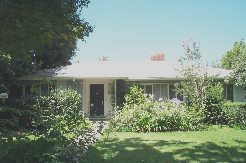
\includegraphics[width=\textwidth]{graphics/calhouse_0230.jpg}
    %     \caption{Original Image. $\mathscr{H_Y}=0.207231$, $SSIM_R=1$, $SSIM_G=1$, $SSIM_B=1$}
    %     \label{fig:casa1original}
    % \end{subfigure}
    % ~ %add desired spacing between images, e. g. ~, \quad, \qquad, \hfill etc. 
    %   %(or a blank line to force the subfigure onto a new line)
    % \begin{subfigure}[t]{0.45\textwidth}
    %     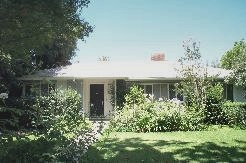
\includegraphics[width=\textwidth]{graphics/calhouse_0230_20-25165283474-10.jpg}
    %     \caption{Enhanced Image. $\mathscr{H_Y}=0.611275$, $SSIM_R=0.00897331$, $SSIM_G=0.00823064$, $SSIM_B=0.00851013$}
    %     \label{fig:casa1enhanced1}
    % \end{subfigure} \\
    ~ %add desired spacing between images, e. g. ~, \quad, \qquad, \hfill etc. 
    %(or a blank line to force the subfigure onto a new line)
    \begin{subfigure}[t]{0.45\textwidth}
    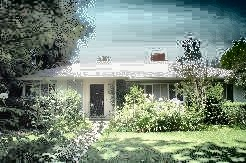
\includegraphics[width=\textwidth]{graphics/calhouse_0230_20-62968204656-00.jpg}
    \caption{Imagen contrastada utilizando $CMOPSO-CLAHE$.  $\mathscr{H_Y}=7,9649405$, $SSIM_R=0,583224$, $SSIM_G=0,596364$, $SSIM_B=0,582346$}
    \label{fig:casa1enhanced2}
    \end{subfigure} 
    \begin{subfigure}[t]{0.45\textwidth}
    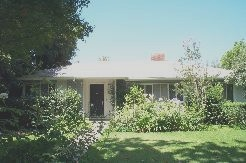
\includegraphics[width=\textwidth]{graphics/calhouse_0230_20-20-0020072469292179818.jpg}
    \caption{Imagen mejorada. $\mathscr{H_Y}=7,211073$, $SSIM_R=0,999795857$, $SSIM_G=0,9999473525$, $SSIM_B=0,99994818587$}
    \label{fig:casa1enhanced3}
    \end{subfigure}

    \caption{Imágenes original y contrastadas para \texttt{calhouse\_230.jpg}}\label{fig:casa1}
    \end{figure}

    \end{frame}


\begin{frame}
\frametitle{Resultados y discusión} 
% \framesubtitle{And also some blocks.} 

\begin{figure}[H]
\centering
    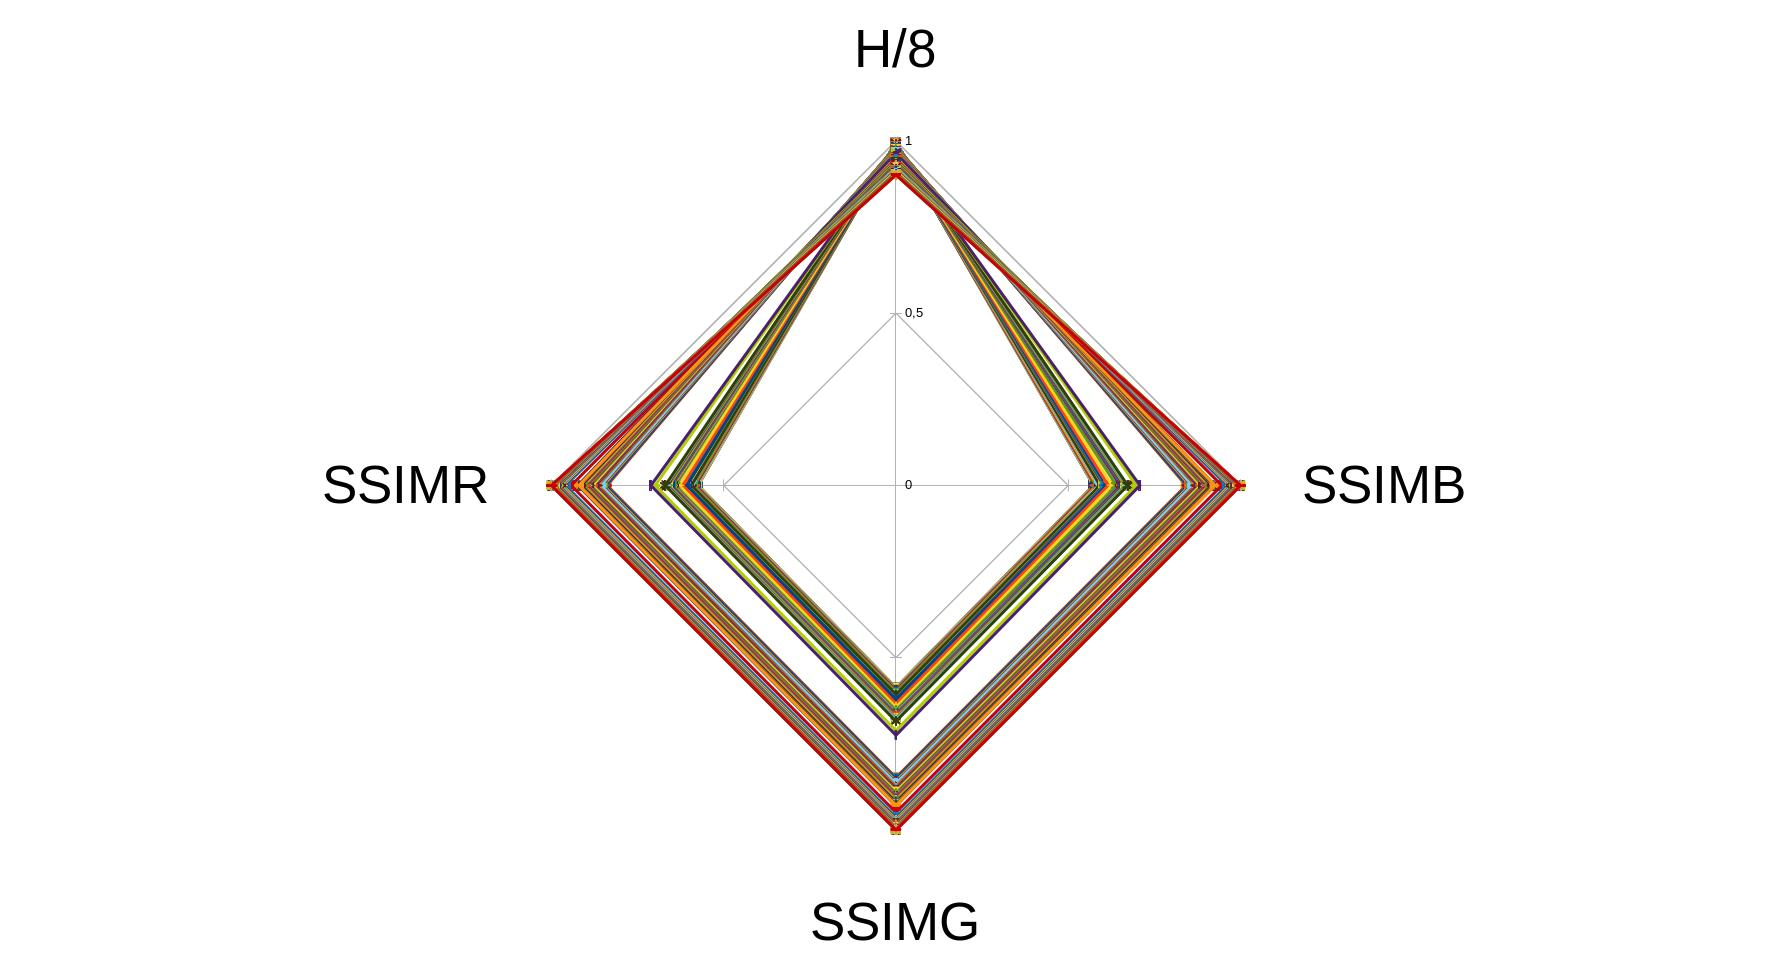
\includegraphics[width=\textwidth]{graphics/calhouse_230_2.jpg}
    \caption{Gráfica de Frente Pareto para las variables de decisión obtenidas para la imagen \texttt{calhouse\_230.jpg}}
    \label{fig:casa1enhancedfp}
\end{figure}

\end{frame}


\begin{frame}
\frametitle{Resultados y discusión} 
% \framesubtitle{And also some blocks.} 
\begin{table}[H]
\setlength{\abovecaptionskip}{2pt plus 3pt minus 2pt} % Chosen fairly arbitrarily
\caption[Parámetros de entrada para $MOPSO$]{Tabla de análisis de correlación entre métricas.}
\begin{center}
\begin{tabular}{||c | c c c c||} 
\hline
Métricas & $\mathscr{H_Y}$ & $SSIM_R$ & $SSIM_G$ & $SSIM_B$ \\ 
\hline
$\mathscr{H_Y}$ & 1 &   &   &  \\ 
\hline
$SSIM_R$ & -0.9826  & 1 &  &  \\ 
\hline
$SSIM_G$ & -0.9823 & 0.9999   & 1   &  \\ 
\hline
$SSIM_B$ & -0.9826 & 0.9999   & 0.9999   & 1 \\ 
\hline
\end{tabular}
\end{center}
\label{table:correlacion}
\end{table}

\begin{itemize}
\item Se puede notar la correlación positiva fuerte entre métricas de similaridad,
\item Además se evidencia una correlación negativa entre la métrica de entropía y las de similaridad,
\item Ésto se reproduce en todas las imágenes de prueba.
\end{itemize}

\end{frame}

\begin{frame}
\frametitle{Resultados y discusión} 
% \framesubtitle{And also some blocks.} 
\begin{exampleblock}{}

\begin{itemize}
	\item Se encontraron parámetros solución con la mejor relación contraste/distorsión
	\item Se encontraron entre 100 y 250 soluciones no dominadas por imagen.
	\item La propuesta supera satisfactoriamente la etapa de prueba de concepto.
	\item La tabla de correlación de métricas sugiere que es posible realizar una implementación de mejora del contraste biobjetivo utilizando el canal de luminancia $Y$ de $YCbCr$
\end{itemize}

\end{exampleblock}

\end{frame}



\section{Conclusiones}

\begin{frame}
\frametitle{Conclusiones} 
% \framesubtitle{And also some blocks.} 
\begin{exampleblock}{}
\begin{itemize}
	\item La implementación propuesta demuestra ser satisfactoria para la realización de Mejora del Contraste Automática.
	\item Se obtienen los parámetros con la mejor relación inversa entre contraste/distorsión.
	\item La implementación es adecuada para la obtención de parámetros del algoritmo de mejora del contraste, aplicados sobre una imagen determinada.
\end{itemize}
\end{exampleblock}
\end{frame}


\section{Trabajos Futuros}

\begin{frame}
\frametitle{Trabajos futuros} 
% \framesubtitle{And also some blocks.} 
\begin{exampleblock}{}
\begin{itemize}
	\item Experimentar utilizando un enfoque de Mejora del Contraste de imágenes a color Biobjetivo basado en el canal de intensidades de alguna representación de color de imágenes digitales.
	\item Experimentar la Mejora de Contraste basada en Metaheurísticas utilizando métricas más adecuadas para la medición de la información de color de la imagen.
	\item Buscar mejoras en la eficiencia de los algoritmos de mejora de Contraste Basado en Metaheurísticas, en base a implementaciones de GPU, nuevas restricciones de las poblaciones de prueba, además de la cantidad de iteraciones impuestas a la metaheurística.
\end{itemize}
\end{exampleblock}
\end{frame}

\begin{frame}
\frametitle{Trabajos futuros} 
% \framesubtitle{And also some blocks.} 
\begin{exampleblock}{}
\begin{itemize}
	\item Experimentar utilizando un enfoque de Mejora del Contraste de imágenes a color con metaheurísticas robustas.
	\item Buscar implementaciones que eviten el ``efecto halo'' detectado en ciertas imágenes que se obtienen como resultado de la propuesta.
	\item Buscar mejoras en la eficiencia de la implementación de La Mejora del Contraste basada en metaheurísticas, de manera a poder entrenar con imágenes de mayor tamaño.
\end{itemize}
\end{exampleblock}
\end{frame}

\begin{frame}
\frametitle{Congresos}  
\begin{exampleblock}{}
 Los resultados del trabajo se presentaron en los siguientes congresos:
\end{exampleblock}
\begin{columns}[onlytextwidth]
\begin{column}{.45\textwidth}
\begin{figure}
  
\includegraphics[width=\textwidth]{graphics/Flyer-CCIS-2016v6.png}
  \caption{4th Conference of Computational Interdisciplinary Sciences - São José Dos Campos - Brasil - 2016}
\end{figure}
\end{column}
\hfill
\begin{column}{.45\textwidth}
		\begin{figure}
		  
\includegraphics[width=\textwidth]{graphics/LOGO-MICAI-2015-OK.jpg}
		  \caption{Mexican Internactional Conference of Artificial Intelligence - Ensenada, Baja California - México - 2017}
		\end{figure}
\end{column}
\end{columns}
\end{frame}

% \begin{frame}{Other blocks}

% Here we display examples of \texttt{abstract}, \texttt{verse}, \texttt{quotation}, and \texttt{quote}.

% \vskip 0.5cm

% \begin{abstract}
% This is an abstract.
% \end{abstract}
% \begin{verse}
% This is a verse.
% \end{verse}
% \begin{quotation}
% This is a quotation.

% \raggedleft -Han Solo
% \end{quotation}
% \begin{quote}
% A quote this is.

% \raggedleft -Yoda
% \end{quote}

% \end{frame}

% \begin{frame}[fragile]
% \frametitle{Bibliography}

% You can cite an article
% \begin{itemize}
% \item normally using \texttt{\textbackslash cite}, e.g.: (\cite{article1})
% \item or display the full citation using \texttt{\textbackslash fullcite}, e.g.:  \fullcite{article1}
% \end{itemize}

% \vskip 0.5cm
% Look at the code of the following slide to see how to automatically split the bibliography on many slides. You can also use \texttt{\textbackslash nocite\{*\}} to display the non-cited publications as well.

% \end{frame}

% \begin{frame}[t,allowframebreaks]
% \frametitle{Bibliography}

% \nocite{*} % will display the non-cited publications as well. Useful for a publication list.

% \printbibliography

% \end{frame}

%\section{Bonus Commands}

% \begin{frame}[fragile]
% \frametitle{Framecard}

% You can display a frame with a colored background and a huge text in the center using the command \texttt{\textbackslash framecard}.
% \vskip 0.5cm 
% For example, you can write:
% \begin{verbatim}
% \framecard{A SECTION\\TITLE}
% \end{verbatim}

% This will display a frame with a orange background and the phrase "A SECTION TITTLE" in the center. You can also use a custom color with \texttt{\textbackslash framecard}:
% \begin{verbatim}
% \framecard{A SECTION\\TITLE}
% \framecard[UniBlue]{A SECTION TITLE\\
% WITH A CUSTOM COLOR}
% \end{verbatim}
% You can see the results of the commands above in the following slides.

% \end{frame}

% \framecard{A SECTION\\TITLE}
% \framecard[UniBlue]{A SECTION TITLE\\WITH A CUSTOM COLOR}

% \begin{frame}[fragile]
% \frametitle{Framepic}

% You can display a frame with a background image using the command \texttt{\textbackslash framepic}. The image will be \textbf{adapted vertically} to fit the the frame. 

% For example, you can write:
% \begin{verbatim}
% \framepic{graphics/darth}{
% 	\framefill
%     \textcolor{white}{Luke,\\I am your supervisor}
%     \vskip 0.5cm
% }
% \end{verbatim}

% Alternatively, to make the background 50\% transparent, you can write \texttt{\textbackslash framepic[0.5]\{graphics/darth\}...}


% You can see the results of the commands above in the following slides.

% \end{frame}


% \framepic{graphics/darth}{
% 	\framefill
%     \textcolor{white}{Luke,\\I am your supervisor}
%     \vskip 0.5cm
% }

% \framepic[0.5]{graphics/darth}{
% 	\vfill
%     \begin{flushright}
%     \textcolor{red}{\textbf{Right-aligned text with\\Semi-transparent background}}
%     \end{flushright}	
% }

% \begin{frame}[t,fragile,allowframebreaks]
% \frametitle{Other bonus commands}

% We provide two other bonus commands:
% \begin{description}
% \item[\texttt{pdfnewline}] you can use \texttt{\textbackslash pdfnewline} to avoid the annoying \texttt{hyperref} related warnings when using newlines in the document's title, author, etc. For example, in this presentation the author is defined as:
% \begin{verbatim}
% \author[Luke Skywalker]{
%   Luke Skywalker, Ph.D.
%   \pdfnewline
%   \texttt{luke.skywalker@uniud.it}
% }
% \end{verbatim}
% \item[\texttt{marker}] you can use \texttt{\textbackslash marker} to highlight some text. The default color is \marker{orange}, but you can also \marker[UniBlue]{use a custom color}. For example:
% \begin{verbatim}
% \marker{Default color}
% \marker[UniBlue]{Custom Color}
% \end{verbatim}
% \item[\texttt{framefill}] you can use \texttt{\textbackslash framefill} to put the text at the bottom of a slide by filling all the vertical space.
% \end{description}

% \end{frame}

\end{document}